% =================================================================================================
% File:			server_tier.tex
% Description:	Defiinisce la sezione relativa al back-end dell'applicazione
% Created:		2015-03-27
% Author:		Tesser Paolo
% Email:		tesser.paolo@mashup-unipd.it
% =================================================================================================
% Modification History:
% Version		Modifier Date		Change											Author
% 0.0.1 		2015-03-27 			creato scheletro								Tesser Paolo
% =================================================================================================
% Version		Modifier Date		Change											Author
% 0.0.2		2015-04-04 				iniziata stesura classi							Nicola F. Lorenzo C.
% =================================================================================================
% Version		Modifier Date		Change											Author
% 0.0.3		2015-04-07 				continuata stesura classi						Nicola F. Luca S.
% =================================================================================================


% CONTENUTO DEL CAPITOLO

\subsection{Server (Back-end)} % (fold)
\label{sub:server}

  \subsubsection{bdsm\_app::server} % (fold)
  [TO DO] (diagramma) \newline \newline

  \begin{itemize}
    \item \textbf{Descrizione}: è il package che racchiude tutte le parti del back-end. \'E quindi l'insieme dei componenti che si occupa di soddifare le richieste provenienti dal front-end, interagire col database, raccogliere i dati provenienti dai social networks, elaborarli ed esporli attraverso servizi REST.
    \item \textbf{Package contenuti}:
      \begin{itemize}
        \item *::server::processor
        \item *::server::db
        \item *::server::miner
        \item *::server::endpoints
      \end{itemize}
    \item \textbf{Interazione con altri componenti}: interagisce con il client definito nella sezione \ref{sub:client} tramite i servizi REST offerti dal modulo in questione;
  \end{itemize}
  % subsubsection bdsm_app_client (end)

  \pagebreak

  % PACKAGE DELLA DB
  % =================================================================================================
% File:			server_tier/db.tex
% Description:	Definisce la sezione relativa al back-end dell'applicazione
% Created:		2015-04-07
% Author:		Cusinato Giacomo
% Email:		cusinato.giacomo@mashup-unipd.it
% =================================================================================================
% Modification History:
% Version		Modifier Date		Change											Author
% 0.0.1			2015-04-18			Modifica grafici e relative descrizioni			Luca Santacatterina
% 0.0.2			2015-05-20			Inserim. descrizione attributi e sist. grafici	Luca Santacatterina
% =================================================================================================

% CONTENUTO DEL CAPITOLO

\subsubsection{server::db} % (fold)
\label{ssub:bdsm_app_server_db}
	\begin{figure}[htbp]
		\centering
		\centerline{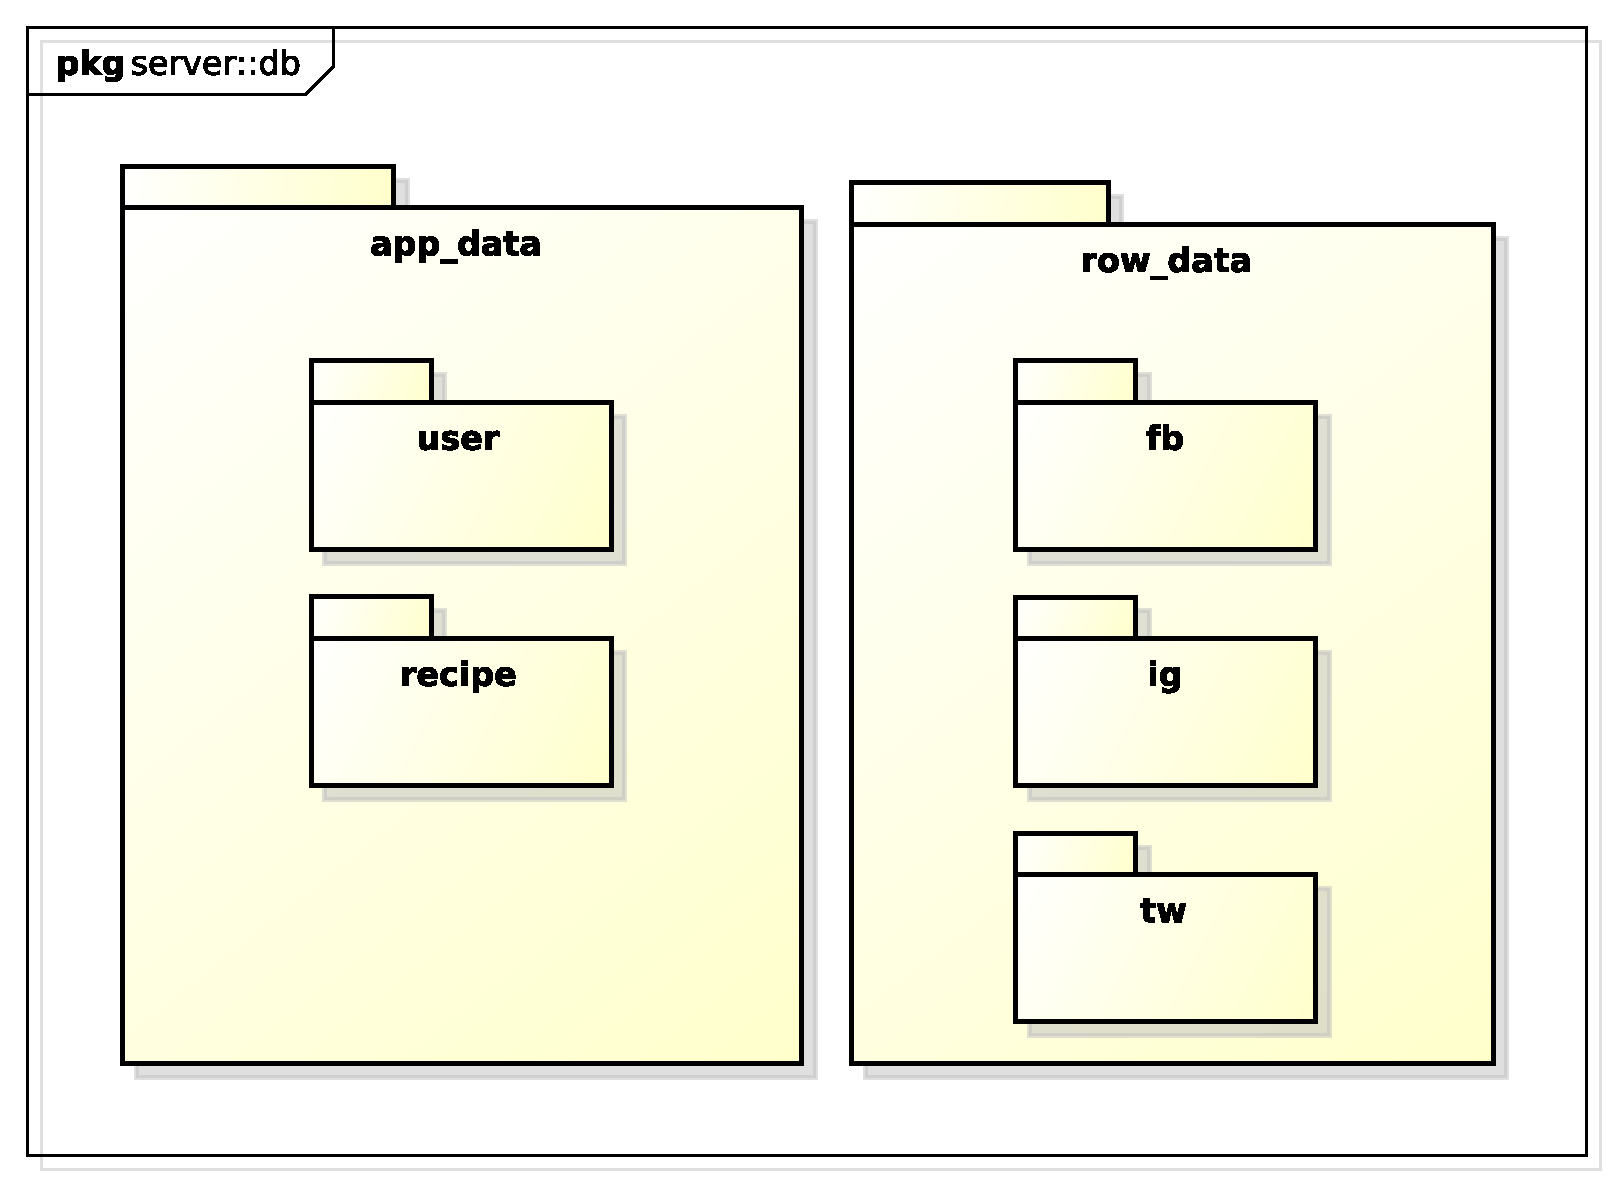
\includegraphics[scale=0.5]{./images/server/db.pdf}}
		\caption{Package - server::db}
	\end{figure}
	\begin{itemize}
		\item \textbf{Descrizione}: è il package che contiene le componenti che gestiscono e mantengono coerente la base di dati. Esse utilizzano standard proprietari Google per la loro implementazione. Sono suddivise in due package: uno atto a rappresentare il modello dei dati grezzi, l'altro per parametri del software e degli utenti;
		\item \textbf{Padre}: server;
		\item \textbf{Package contenuti}:
			\begin{itemize}
				\item server::app\_data.
				\item server::raw\_data;
			\end{itemize}
	\end{itemize}

% subsubsection RAW_DATA
\subsubsection{server::db::raw\_data} % (fold)
\label{ssub:bdsm_app_server_raw_data}
	\begin{figure}[htbp]
		\centering
		\centerline{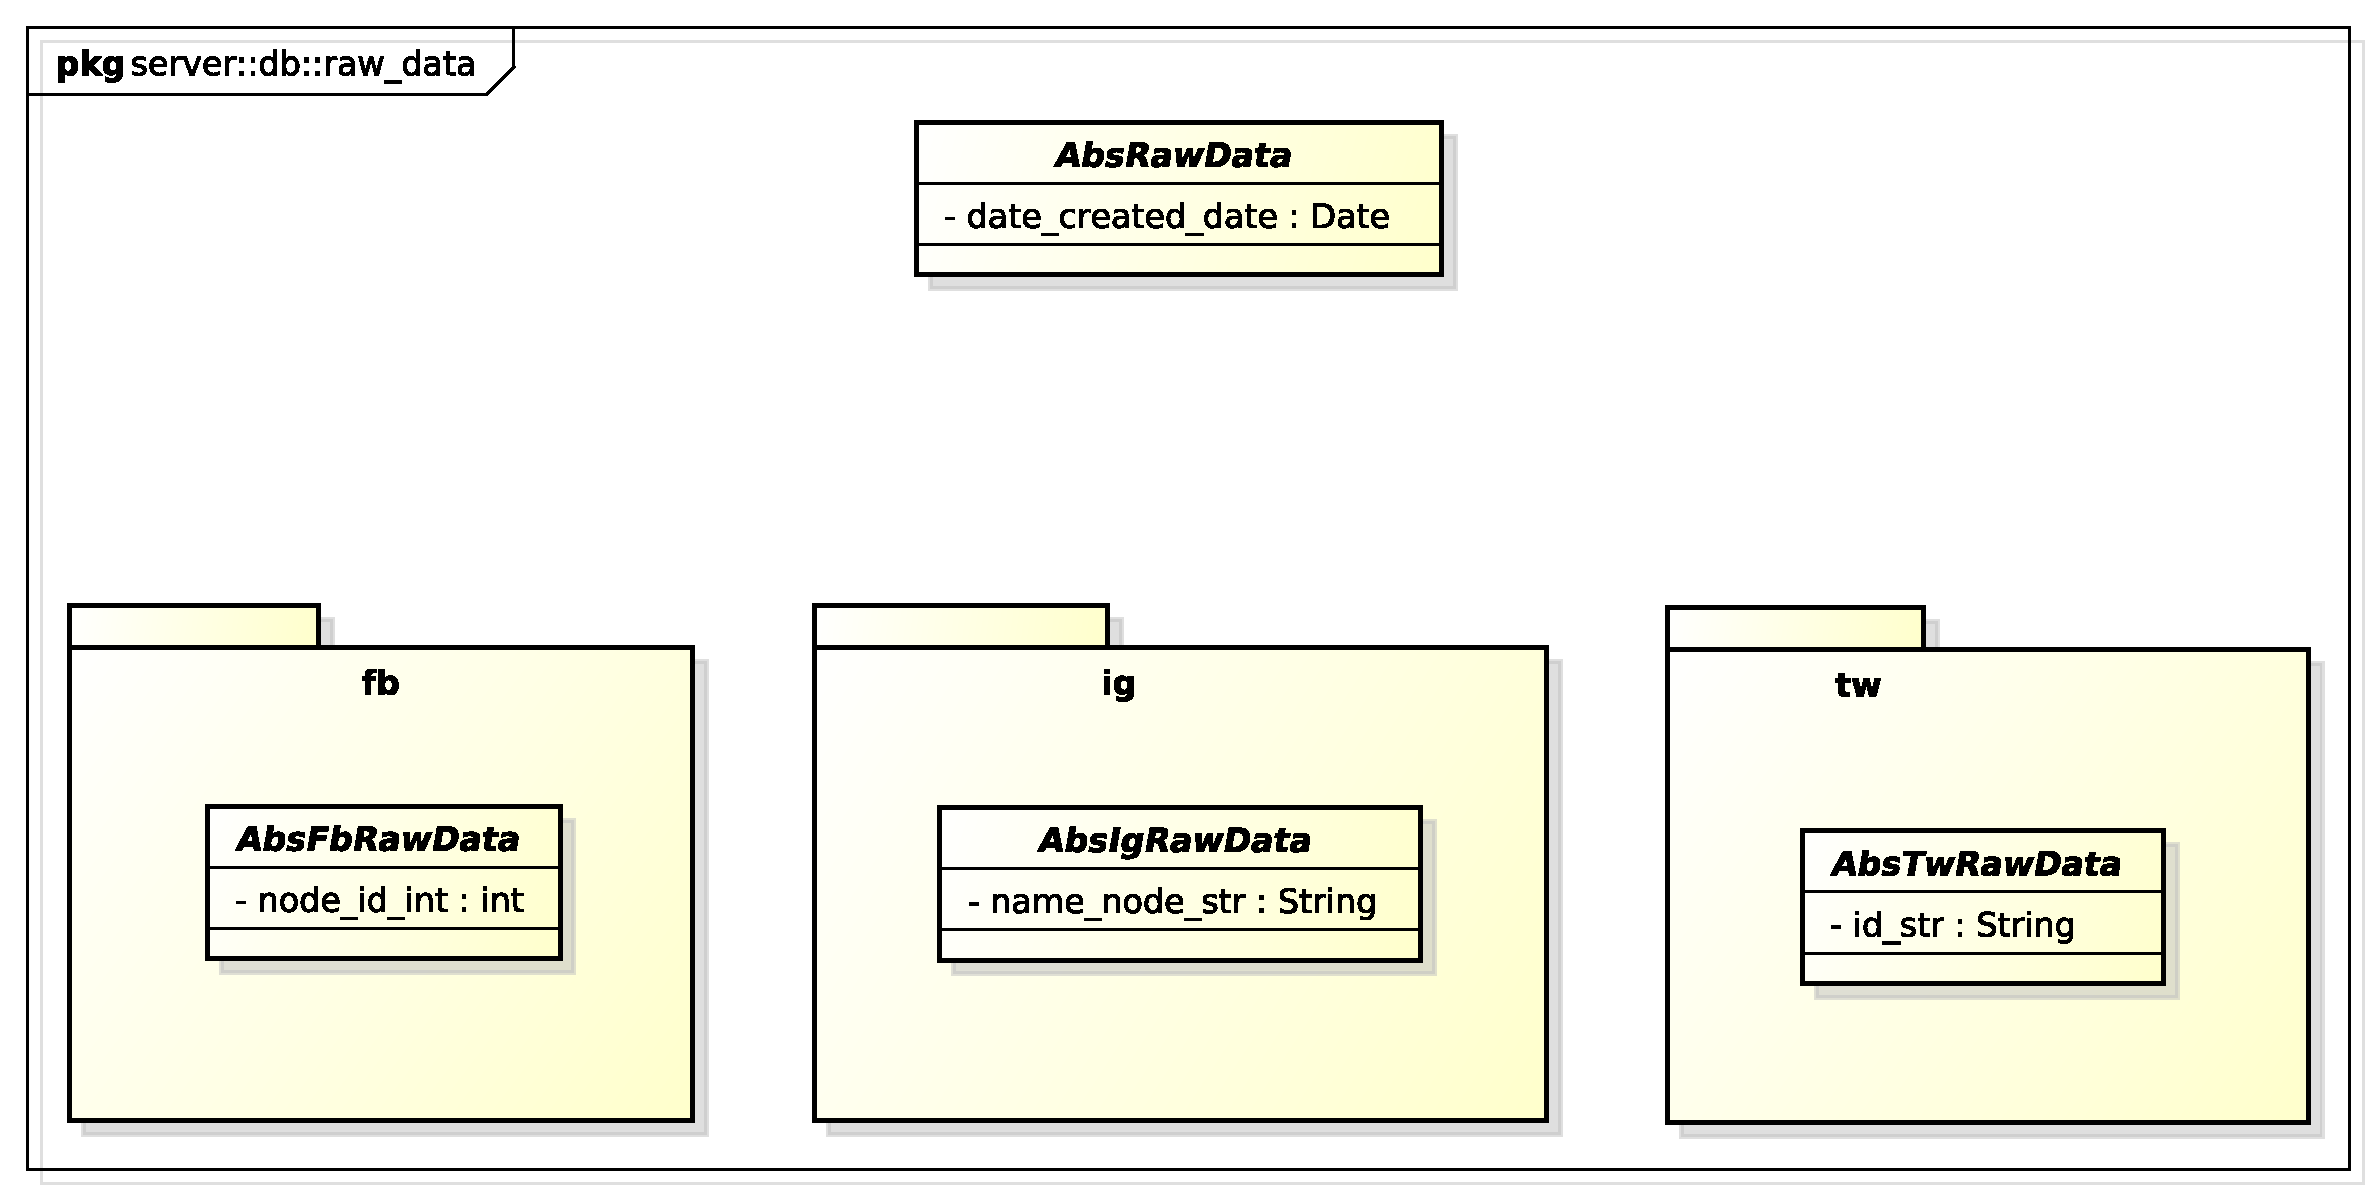
\includegraphics[scale=0.4]{./images/server/raw_data.pdf}}
		\caption{Package - server::db::raw\_data}
	\end{figure}
	\begin{itemize}
	\item \textbf{Descrizione}: package che definisce il modello dei dati grezzi ricavati dai vari social network;
		\item \textbf{Padre}: server::db;
		\item \textbf{Package contenuti}:
			\begin{itemize}
				\item server::db::raw\_data::fb
				\item server::db::raw\_data::tw
				\item server::db::raw\_data::ig
		\end{itemize}
	\end{itemize}

	\paragraph{Classi} % (fold)
		\subparagraph{server::db::raw\_data::AbsRawData} % (fold)
		\label{subp:bdsm_app_server_raw_data_absrawdata}
			\begin{itemize}
				\item \textbf{Descrizione}: classe astratta che definisce il modello di un dato grezzo;
				\item \textbf{Utilizzo}: la classe funge da padre per tutte le classi rappresentanti un dato grezzo;
				\item \textbf{Relazioni con altre classi}:
					\begin{itemize}
						\item server::db::raw\_data::fb::AbsFbRawData
						\item server::db::raw\_data::tw::AbsTwRawData
						\item server::db::raw\_data::ig::AbsIgRawData
						\item server::db::raw\_data::fb::RawFbPageTrend
						\item server::db::raw\_data::fb::RawFbEventTrend
						\item server::db::raw\_data::fb::RawFbPostTrendTrend
						\item server::db::raw\_data::tw::RawTwUserTrend
						\item server::db::raw\_data::tw::RawTwUserTweet
						\item server::db::raw\_data::ig::RawIgUserTrend
						\item server::db::raw\_data::ig::RawIgHashtagTrend
						\item server::db::raw\_data::ig::RawIgMedia
					\end{itemize}
				\item \textbf{Attributi}:
					\begin{itemize}
						\item \textcolor{forestgreen}{\texttt{+ date\_created\_date : Date}}
						\begin{description}
							\item \textbf{Descrizione}: data acquisizione dati grezzi
						\end{description}
					\end{itemize}
				\item \textbf{Metodi}: N/A
			\end{itemize}

		% subsubsection FACEBOOK
		\subsubsection{server::db::raw\_data::fb} % (fold)
		\label{ssub:bdsm_app_server_db_raw_data_fb}
		\begin{figure}[htbp]
			\centering
			\centerline{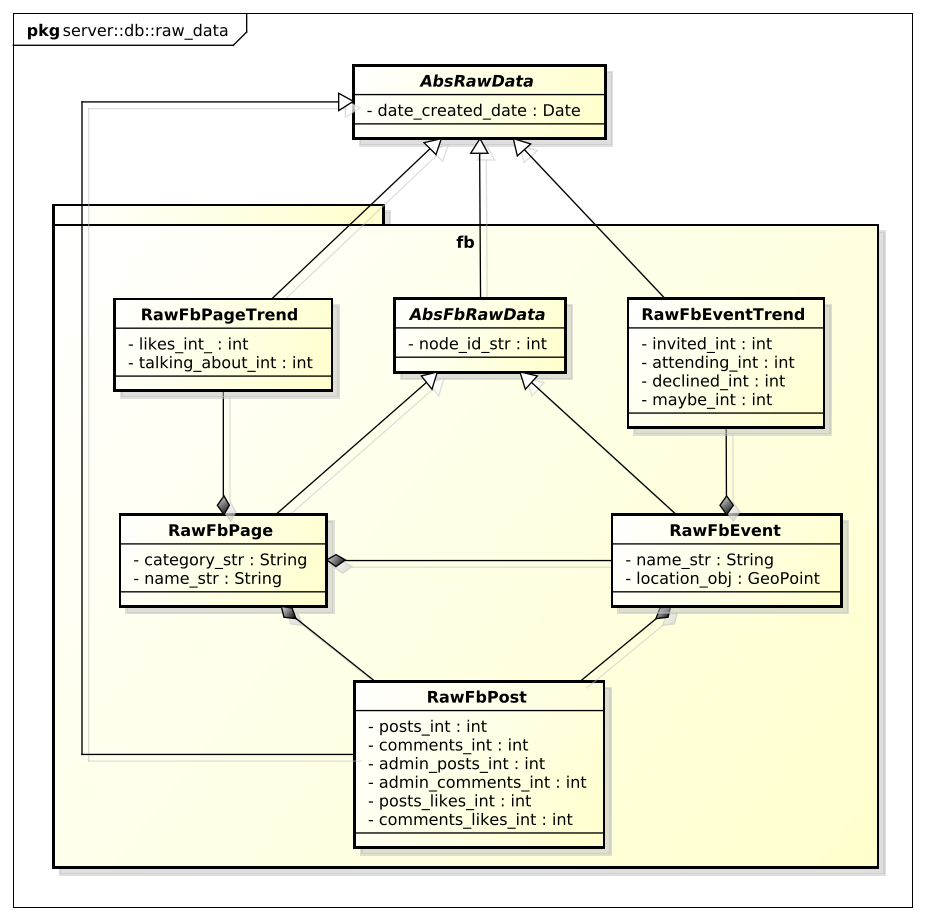
\includegraphics[scale=0.5]{./images/server/raw_data_fb.pdf}}
			\caption{Package - server::db::raw\_data::fb}
		\end{figure}
		\begin{itemize}
		  \item \textbf{Descrizione}:  è il package contenente le classi che definiscono i modelli dei dati grezzi relativi a Facebook;
		  \item \textbf{Padre}: server::db::raw\_data
		  \item \textbf{Interazione con altri componenti}:
		  	\begin{itemize}
		  		\item server::db
			\end{itemize}
		\end{itemize}
		% subsubsection

		\paragraph{Classi} % (fold)
			\subparagraph{server::db::raw\_data::fb::AbsFbRawData} % (fold)
			\label{subp:server_db_raw_data_fb_absfbrawdata}
				\begin{figure}[htbp]
					\centering
					\centerline{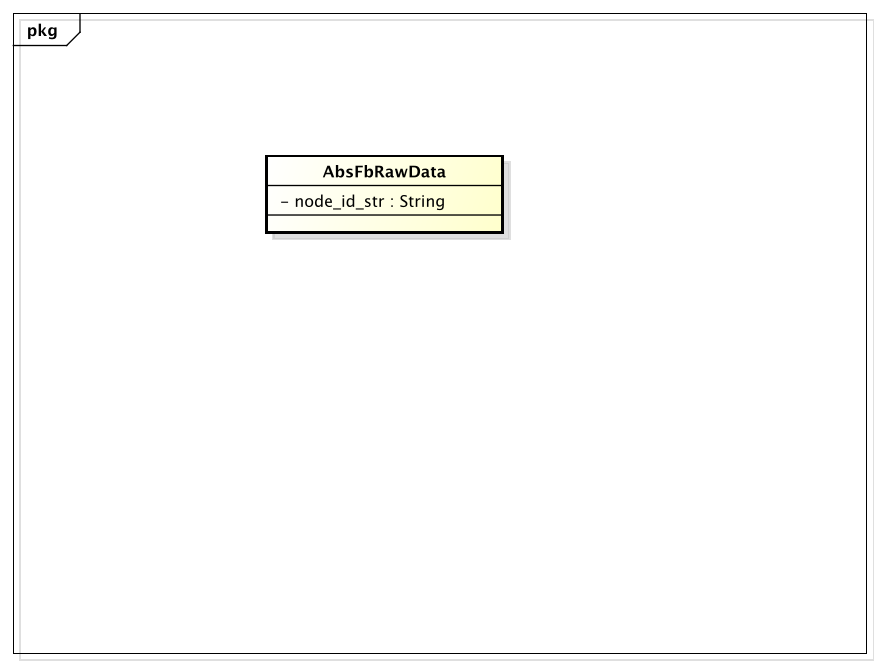
\includegraphics[scale=0.75]{./images/server/classes/db/abs_fb_raw_data.pdf}}
					\caption{Classe - server::db::raw\_data::fb::AbsFbRawData}
				\end{figure}
				\begin{itemize}
					\item \textbf{Descrizione}: classe astratta che definisce il modello dati grezzi relativi a Facebook;
					\item \textbf{Utilizzo}: la classe contiene l'id fornito dall'utente il quale permette di identificare univocamente la risorsa nel social media;
					\item \textbf{Classi ereditate}: server::db::raw\_data::AbsRawData
					\item \textbf{Attributi}:
					\begin{itemize}
						\item \textcolor{forestgreen}{\texttt{+ node\_id\_str : String}}
						\begin{description}
							\item \textbf{Descrizione}: codice identificativo di un evento o di una pagina Facebook.
						\end{description}
					\end{itemize}
					\item \textbf{Metodi}: N/A
				\end{itemize}
			% subparagraph server_db_raw_data_fb_absfbrawdata [end]


			\subparagraph{server::db::raw\_data::fb::RawFbPage} % (fold)
			\label{subp:server_db_raw_data_fb_rawfbpage}
				\begin{figure}[htbp]
					\centering
					\centerline{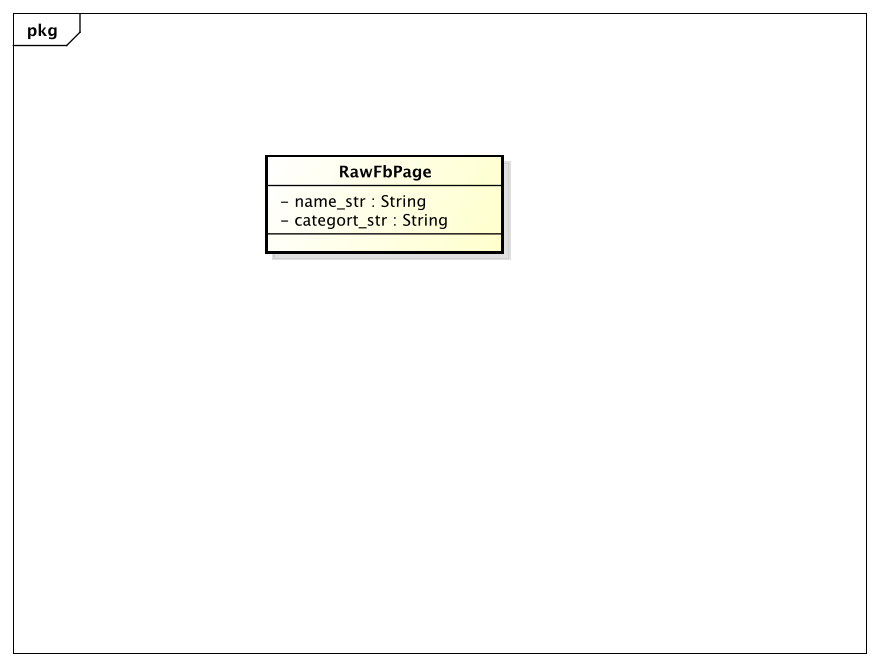
\includegraphics[scale=0.75]{./images/server/classes/db/raw_fb_page.pdf}}
					\caption{Classe - server::db::raw\_data::fb::RawFbPage}
				\end{figure}
				\begin{itemize}
					\item \textbf{Descrizione}: classe che rappresenta il modello di una pagina Facebook;
					\item \textbf{Utilizzo}: la classe fornisce metodi per memorizzare i dati statici di una pagina Facebook;
					\item \textbf{Classi ereditate}: server::db::raw\_data::AbsFbRawData
					\item \textbf{Relazioni con altre classi}:
						\begin{itemize}
							\item server::db::raw\_data::fb::RawFbEvent
							\item server::db::raw\_data::fb::RawFbPageTrend
							\item server::db::raw\_data::fb::RawFbPostTrend
						\end{itemize}
					\item \textbf{Attributi}:
					\begin{itemize}
						\item \textcolor{forestgreen}{\texttt{+ name\_str : String}}
						\begin{description}
							\item \textbf{Descrizione}: nome della pagina Facebook.
						\end{description}
						\item \textcolor{forestgreen}{\texttt{+ category\_str : String}}
						\begin{description}
							\item \textbf{Descrizione}: categoria della pagina Facebook.
						\end{description}
					\end{itemize}
					\item \textbf{Metodi}: N/A
				\end{itemize}
			% subparagraph server_db_raw_data_fb_rawfbpage [end]

			\subparagraph{server::db::raw\_data::fb::RawFbPageTrend} % (fold)
			\label{subp:server_db_raw_data_fb_rowfbpagetrend}
				\begin{figure}[htbp]
					\centering
					\centerline{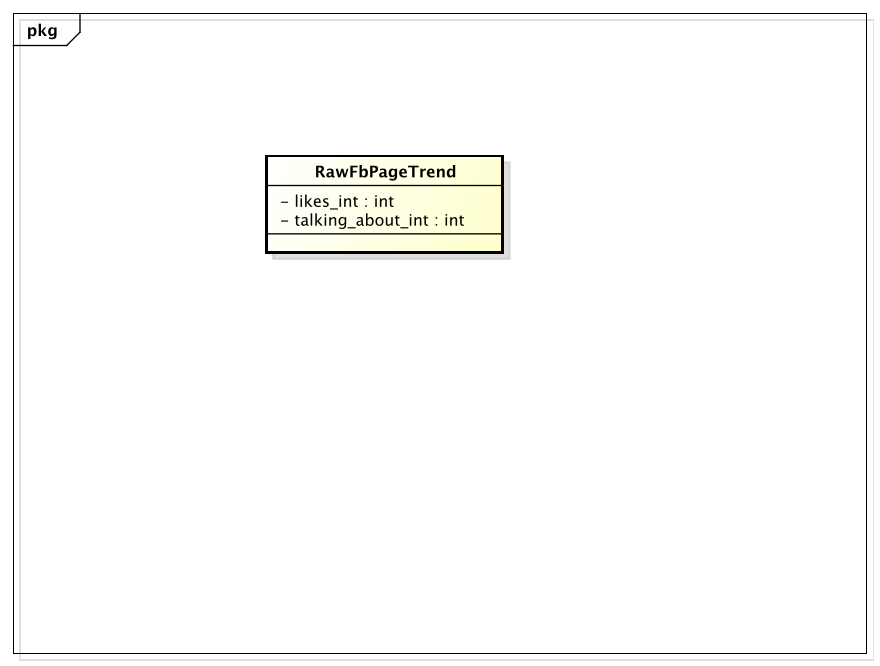
\includegraphics[scale=0.75]{./images/server/classes/db/raw_fb_page_trend.pdf}}
					\caption{Classe - server::db::raw\_data::fb::RawFbPageTrend}
				\end{figure}
				\begin{itemize}
					\item \textbf{Descrizione}: classe che rappresenta il modello del trend dei dati una pagina Facebook;
					\item \textbf{Utilizzo}: la classe viene utilizzata per memorizzare e il numero di like e di talking about di ogni singola pagina. Come per tutti gli oggetti di tipo trend, vengono ricavati i dati fino a 3 giorni prima della creazione dell'oggetto;
					\item \textbf{Classi ereditate}: server::db::raw\_data::AbsRawData
					\item \textbf{Attributi}:
					\begin{itemize}
						\item \textcolor{forestgreen}{\texttt{+ likes\_int : int}}
						\begin{description}
							\item \textbf{Descrizione}: numero dei likes di una determinata pagina Facebook,
						\end{description}
						\item \textcolor{forestgreen}{\texttt{+ talking\_about\_int : int}}
						\begin{description}
							\item \textbf{Descrizione}: numero di talking about di una determinata pagina Facebook.
						\end{description}
					\end{itemize}
					\item \textbf{Metodi}: N/A
				\end{itemize}
			% subparagraph server_db_raw_data_fb_rowfbpagetrend [end]


			\subparagraph{server::db::raw\_data::fb::RawFbEvent} % (fold)
			\label{subp:server_db_raw_data_fb_rawfbevent}
				\begin{figure}[htbp]
					\centering
					\centerline{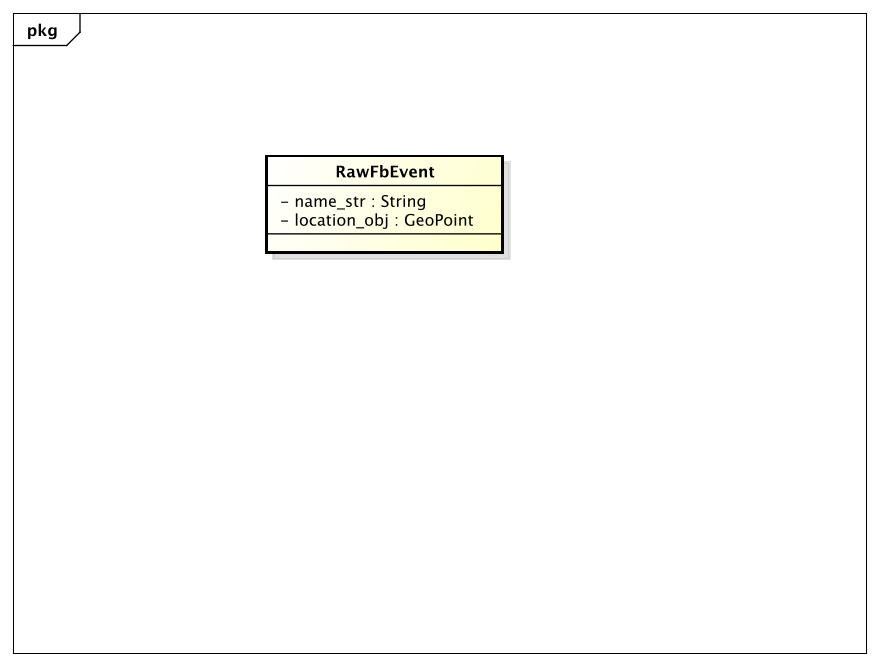
\includegraphics[scale=0.75]{./images/server/classes/db/raw_fb_event.pdf}}
					\caption{Classe - server::db::raw\_data::fb::RawFbEvent}
				\end{figure}
				\begin{itemize}
					\item \textbf{Descrizione}: classe che rappresenta il modello di un evento Facebook;
					\item \textbf{Utilizzo}: la classe fornisce metodi per memorizzare i dati statici di un evento Facebook;
					\item \textbf{Classi ereditate}: server::db::raw\_data::AbsFbRawData
					\item \textbf{Relazioni con altre classi}:
						\begin{itemize}
							\item server::db::raw\_data::fb::RawFbEventTrend
							\item server::db::raw\_data::fb::RawFbPostTrend
						\end{itemize}
					\item \textbf{Attributi}:
					\begin{itemize}
						\item \textcolor{forestgreen}{\texttt{+ name\_str : String}}
						\begin{description}
							\item \textbf{Descrizione}: nome dell'evento Facebook.
						\end{description}
						\item \textcolor{forestgreen}{\texttt{+ location\_obj : GeoPoint}}
						\begin{description}
							\item \textbf{Descrizione}: location dell'evento espressa in latitudine e longitudine.
						\end{description}
					\end{itemize}
					\item \textbf{Metodi}: N/A
				\end{itemize}
			% subparagraph server_db_raw_data_fb_rawfbevent [end]

			\subparagraph{server::db::raw\_data::fb::RawFbEventTrend} % (fold)
			\label{subp:server_db_raw_data_fb_rowfbeventtrend}
				\begin{figure}[htbp]
					\centering
					\centerline{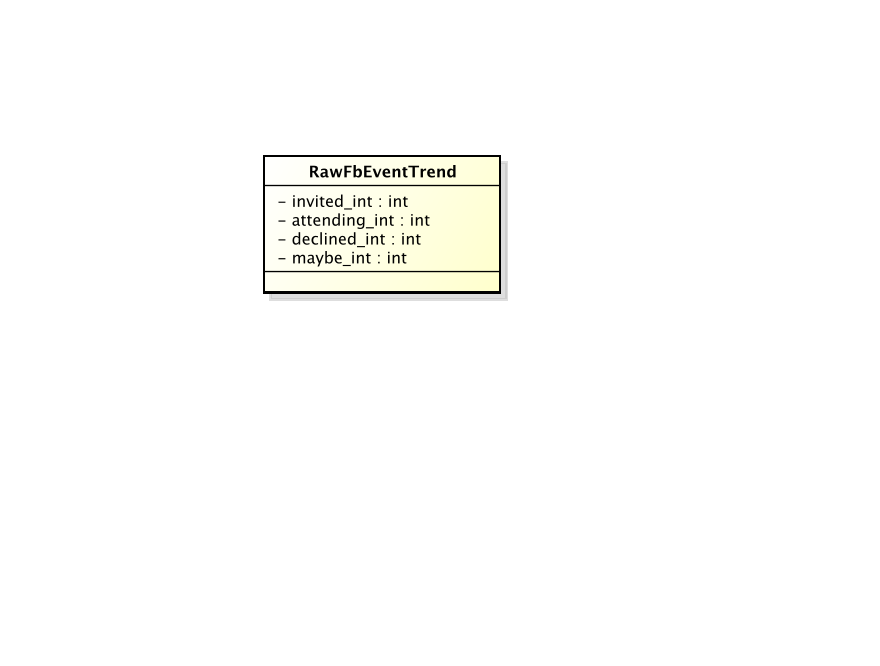
\includegraphics[scale=0.75]{./images/server/classes/db/raw_fb_event_trend.pdf}}
					\caption{Classe - server::db::raw\_data::fb::RawFbEventTrend}
				\end{figure}
				\begin{itemize}
					\item \textbf{Descrizione}: classe che rappresenta il modello del trend di un evento su Facebook;
					\item \textbf{Utilizzo}: la classe viene utilizzata per memorizzare il numero di utenti invitati, partecipanti e non di un evento. Come per tutti gli oggetti di tipo trend, vengono ricavati i dati fino a 3 giorni prima della creazione dell'oggetto;
					\item \textbf{Classi ereditate}: server::db::raw\_data::AbsRawData
					\item \textbf{Attributi}:
					\begin{itemize}
						\item \textcolor{forestgreen}{\texttt{+ invited\_int : int}}
						\begin{description}
							\item \textbf{Descrizione}: numero delle persone invitate all'evento Facebook.
						\end{description}
						\item \textcolor{forestgreen}{\texttt{+ attending\_int : int}}
						\begin{description}
							\item \textbf{Descrizione}: numero persone partecipanti all'evento Facebook
						\end{description}
						\item \textcolor{forestgreen}{\texttt{+ declined\_int : int}}
						\begin{description}
							\item \textbf{Descrizione}: numero persone che hanno rifiutato la partecipazione all'evento Facebook.
						\end{description}
						\item \textcolor{forestgreen}{\texttt{+ maybe\_int : int}}
						\begin{description}
							\item \textbf{Descrizione}: numero persone incerte se partecipare all'evento Facebook.
						\end{description}
					\end{itemize}
					\item \textbf{Metodi}: N/A
				\end{itemize}
			% subparagraph server_db_raw_data_fb_rowfbeventtrend [end]


			\subparagraph{server::db::raw\_data::fb::RawFbPostTrend} % (fold)
			\label{subp:server_db_raw_data_fb_RawFbPostTrend}
				\begin{figure}[htbp]
					\centering
					\centerline{\includegraphics[scale=0.75]{./images/server/classes/db/raw_fb_post_trend.pdf}}
					\caption{Classe - server::db::raw\_data::fb::RawFbPostTrend}
				\end{figure}
				\begin{itemize}
					\item \textbf{Descrizione}: classe che rappresenta il modello del trend dei post di una pagina o di un evento su Facebook;
					\item \textbf{Utilizzo}: viene utilizzata per memorizzare i dati relativi al trend dei post di una pagina o un pagina o evento Facebook. Come per tutti gli oggetti di tipo trend, vengono ricavati i dati fino a 3 giorni prima della creazione dell'oggetto;
					\item \textbf{Attributi}:
					\begin{itemize}
						\item \textcolor{forestgreen}{\texttt{+ posts\_int : int}}
						\begin{description}
							\item \textbf{Descrizione}: numero dei post presenti nella pagina o nell'evento.
						\end{description}
						\item \textcolor{forestgreen}{\texttt{+ comments\_int : int}}
						\begin{description}
							\item \textbf{Descrizione}: numero totale di commenti ai post della pagina o dell'evento.
						\end{description}
						\item \textcolor{forestgreen}{\texttt{+ admin\_posts\_int : int}}
						\begin{description}
							\item \textbf{Descrizione}: numero dei post effettuati esclusivamente da una pagina Facebook e non da terzi.
						\end{description}
						\item \textcolor{forestgreen}{\texttt{+ admin\_comments\_int : int}}
						\begin{description}
							\item \textbf{Descrizione}: numero dei commenti effettuati esclusivamente da una pagina Facebook e non da terzi.
						\end{description}
						\item \textcolor{forestgreen}{\texttt{+ posts\_like\_int : int}}
						\begin{description}
							\item \textbf{Descrizione}: numero totale dei likes ai post di una pagina o evento Facebook.
						\end{description}
						\item \textcolor{forestgreen}{\texttt{+ comments\_like\_int : int}}
						\begin{description}
							\item \textbf{Descrizione}: numero totale ai likes dei commenti presenti nei post di una pagina o evento Facebook.
						\end{description}
					\end{itemize}
					\item \textbf{Metodi}: N/A
				\end{itemize}
			% subparagraph server_db_raw_data_fb_RawFbPostTrend [end]


		% subsubsection TWITTER
		\subsubsection{server::db::raw\_data::tw} % (fold)
		\label{ssub:bdsm_app_server_db_raw_data_tw}
		\begin{figure}[htbp]
			\centering
			\centerline{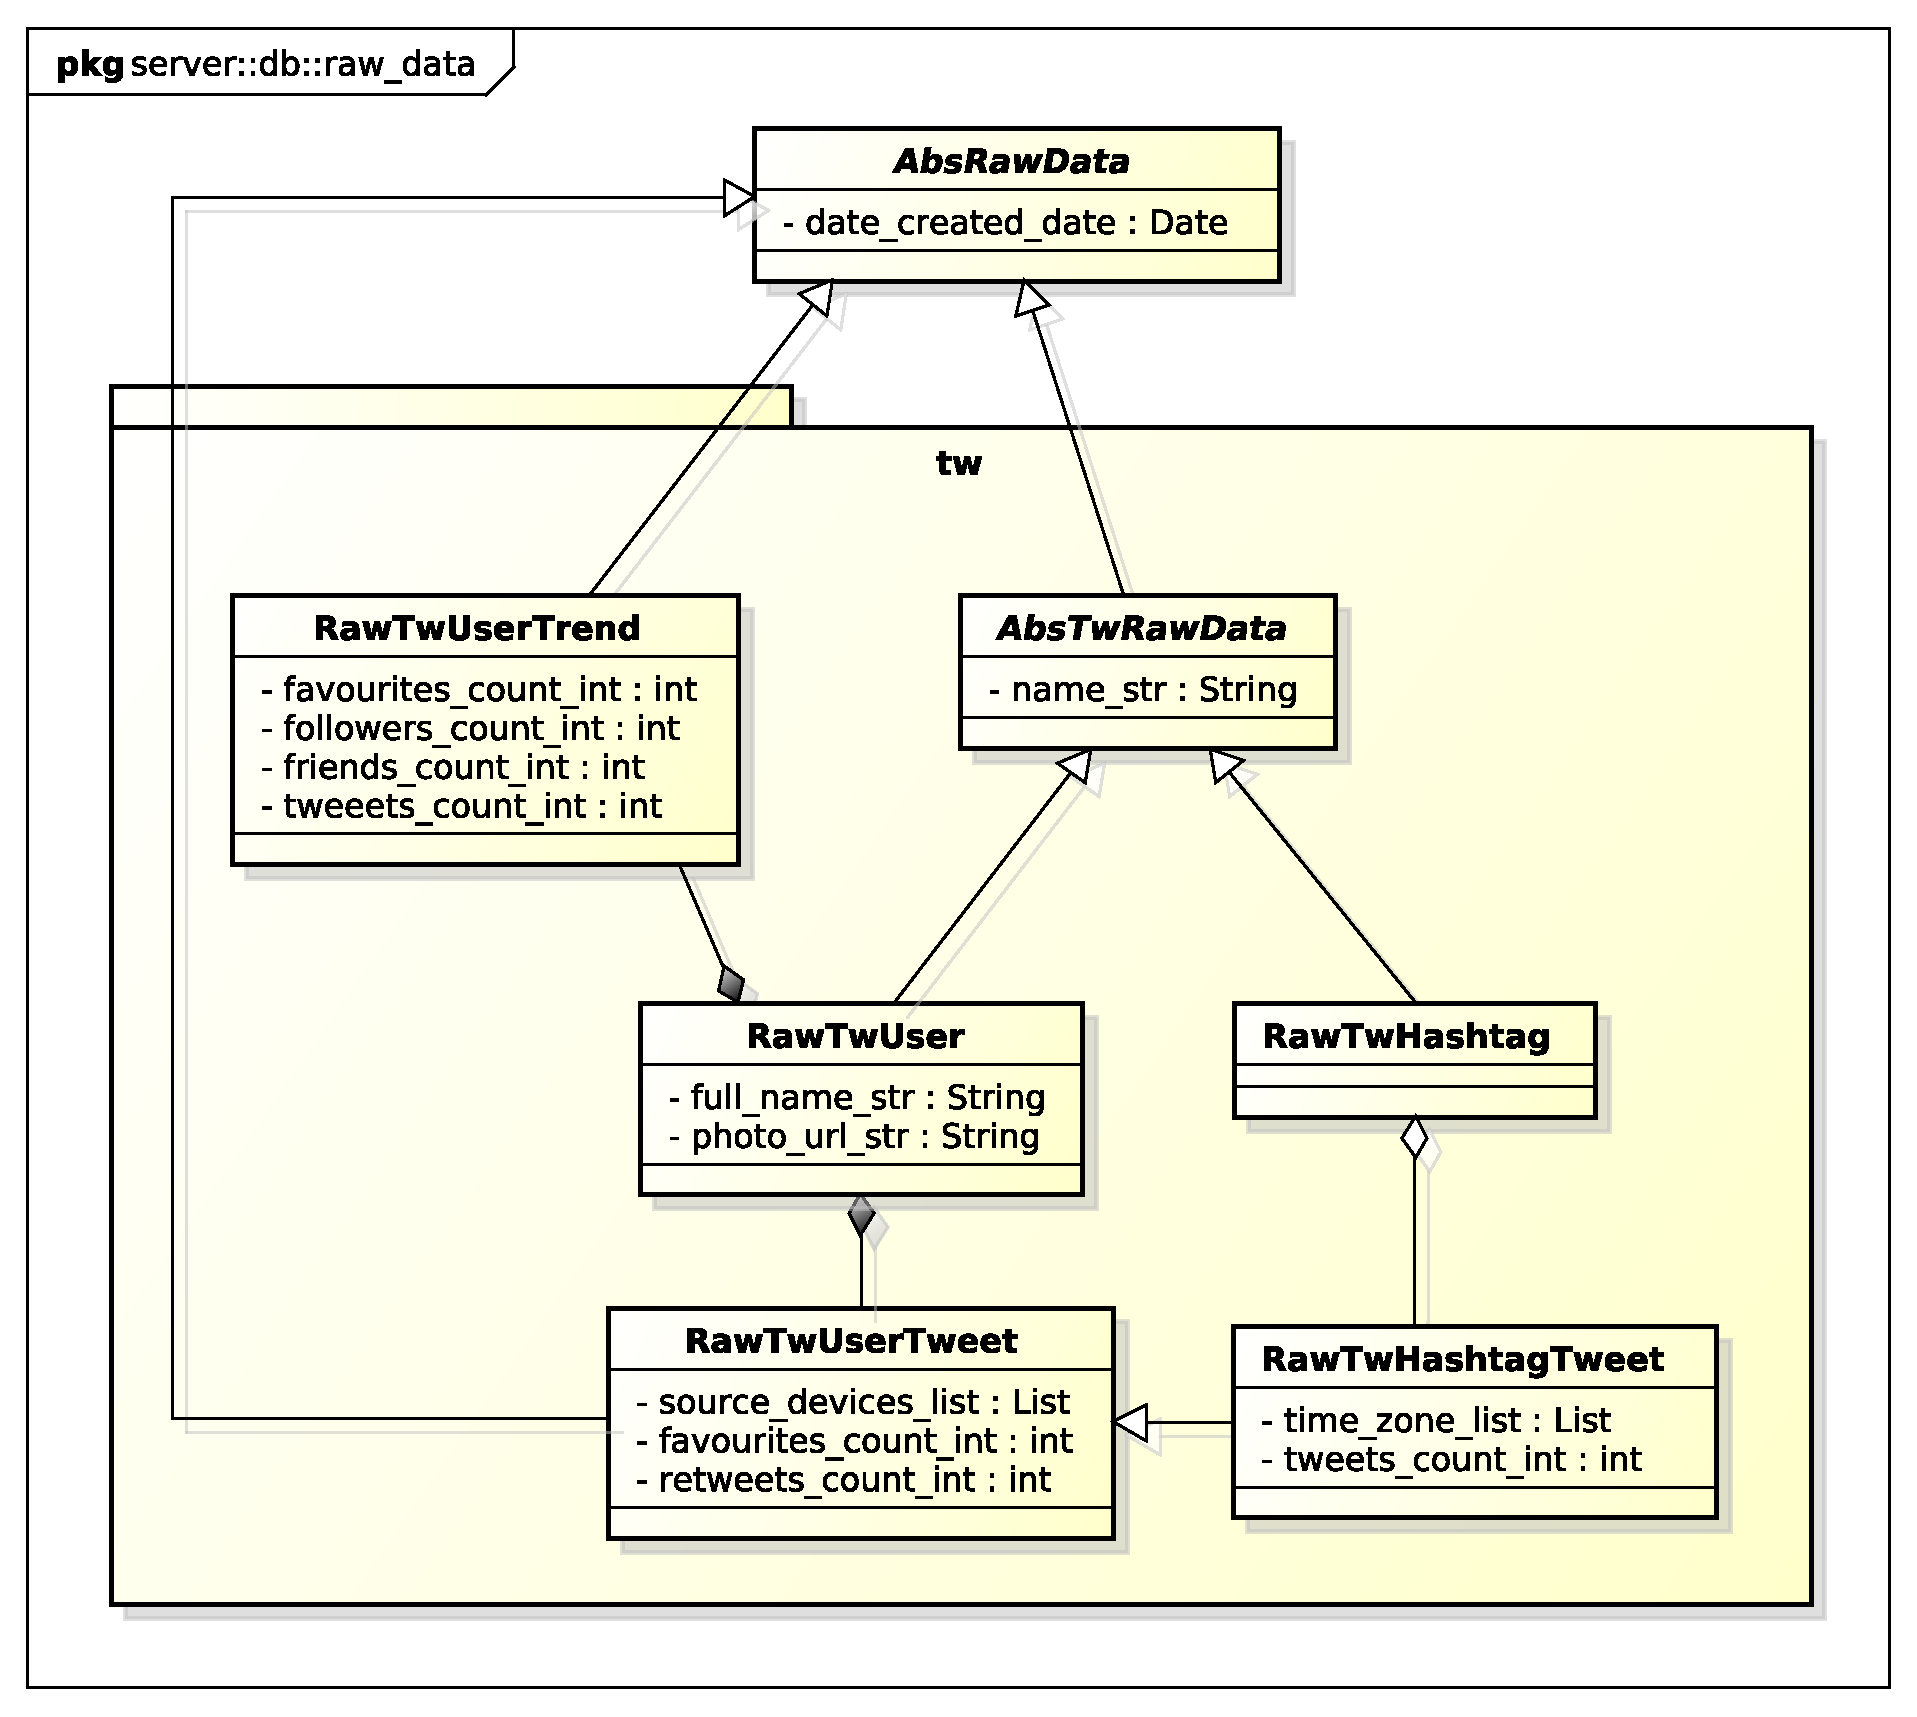
\includegraphics[scale=0.45]{./images/server/raw_data_tw.pdf}}
			\caption{Package - server::db::raw\_data::tw}
		\end{figure}

		\begin{itemize}
		  \item \textbf{Descrizione}: è il package contenente le classi che definiscono i modelli dei dati grezzi relativi a Twitter;
		  \item \textbf{Padre}: server::db::raw\_data
		  \item \textbf{Interazione con altri componenti}:
		  	\begin{itemize}
		  		\item server::db
			\end{itemize}
		\end{itemize}
		% subsubsection

		\paragraph{Classi} % (fold)


		\subparagraph{server::db::raw\_data::tw::AbsTwRawData} % (fold)
		\label{subp:server_db_raw_data_tw_abstwrawdata}
			\begin{figure}[htbp]
				\centering
				\centerline{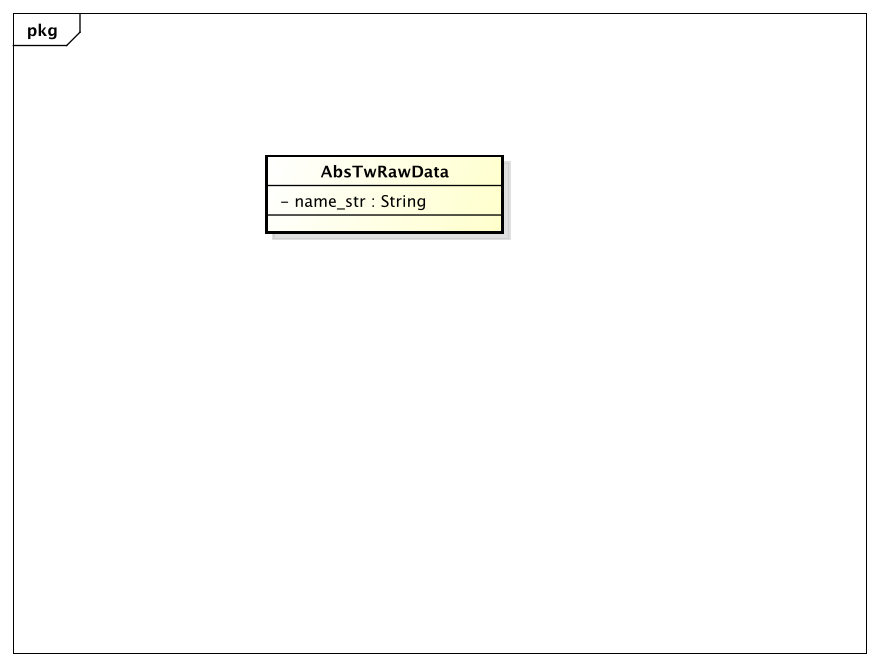
\includegraphics[scale=0.75]{./images/server/classes/db/abs_tw_raw_data.pdf}}
				\caption{Classe - server::db::raw\_data::tw::AbsTwRawData}
			\end{figure}
			\begin{itemize}
				\item \textbf{Descrizione}: classe astratta che definisce il modello dati grezzi relativi a Twitter;
				\item \textbf{Utilizzo}: la classe contiene l'id fornito dall'utente il quale permette di identificare univocamente la risorsa nel social media;
				\item \textbf{Classi ereditate}: server::db::raw\_data::AbsRawData
				\item \textbf{Attributi}:
					\begin{itemize}
						\item \textcolor{forestgreen}{\texttt{+ name\_str : String}}
						\begin{description}
							\item \textbf{Descrizione}: nome identificativo della pagina o dell'hashtag Twitter.
						\end{description}
					\end{itemize}
				\item \textbf{Metodi}: N/A
			\end{itemize}
		% subparagraph server_db_raw_data_tw_abstwrawdata [end]


		\subparagraph{server::db::raw\_data::tw::RawTwUser} % (fold)
		\label{subp:server_db_raw_data_tw_rawtwuser}
			\begin{figure}[htbp]
				\centering
				\centerline{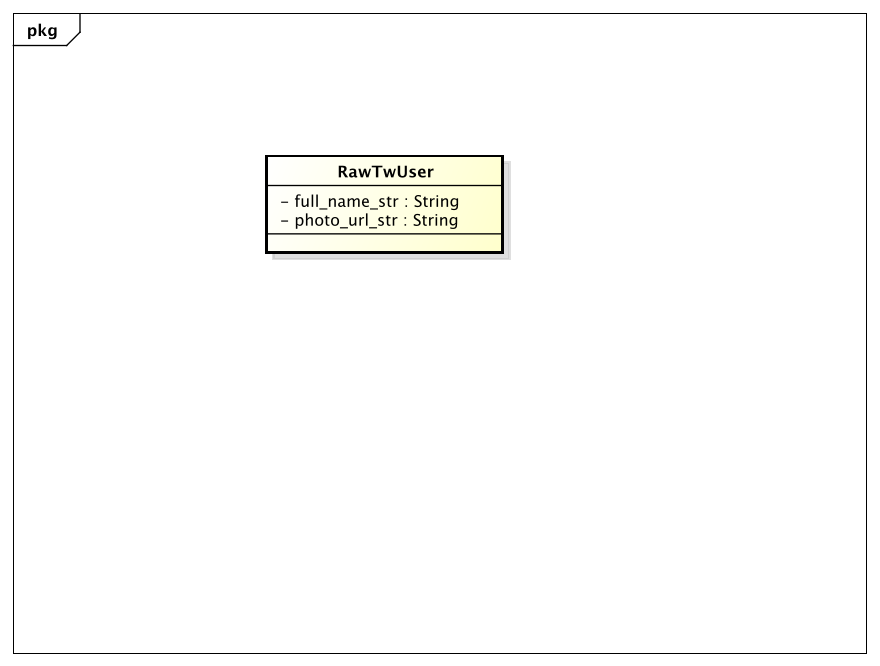
\includegraphics[scale=0.75]{./images/server/classes/db/raw_tw_user.pdf}}
				\caption{Classe - server::db::raw\_data::tw::RawTwUser}
			\end{figure}
			\begin{itemize}
				\item \textbf{Descrizione}: classe che definisce il modello dei dati di un utente Twitter;
				\item \textbf{Utilizzo}: la classe viene utilizzata per fornire una descrizione completa dell'utente Twitter. Vengono forniti metodi automatici per il conteggio dei parametri che verranno utilizzati per seguire un trend;;
				\item \textbf{Classi ereditate}: server::db::raw\_data::AbsTwRawData
				\item \textbf{Relazioni con altre classi}:
					\begin{itemize}
						\item server::db::raw\_data::tw::RawTwUserTrend
						\item server::db::raw\_data::tw::RawTwUserTweet
					\end{itemize}
				\item \textbf{Attributi}:
					\begin{itemize}
						\item \textcolor{forestgreen}{\texttt{+ full\_name\_str : String}}
						\begin{description}
							\item \textbf{Descrizione}: nome completo dell'utente Twitter.
						\end{description}
						\item \textcolor{forestgreen}{\texttt{+ photo\_url\_str : String}}
						\begin{description}
							\item \textbf{Descrizione}: indirizzo url della foto profilo dell'utente Twitter.
						\end{description}
					\end{itemize}
				\item \textbf{Metodi}: N/A
			\end{itemize}
		% subparagraph server_db_raw_data_tw_rawtwuser [end]


		\subparagraph{server::db::raw\_data::tw::RawTwUserTrend} % (fold)
		\label{subp:server_db_raw_data_tw_rawtwusertrend}
			\begin{figure}[htbp]
				\centering
				\centerline{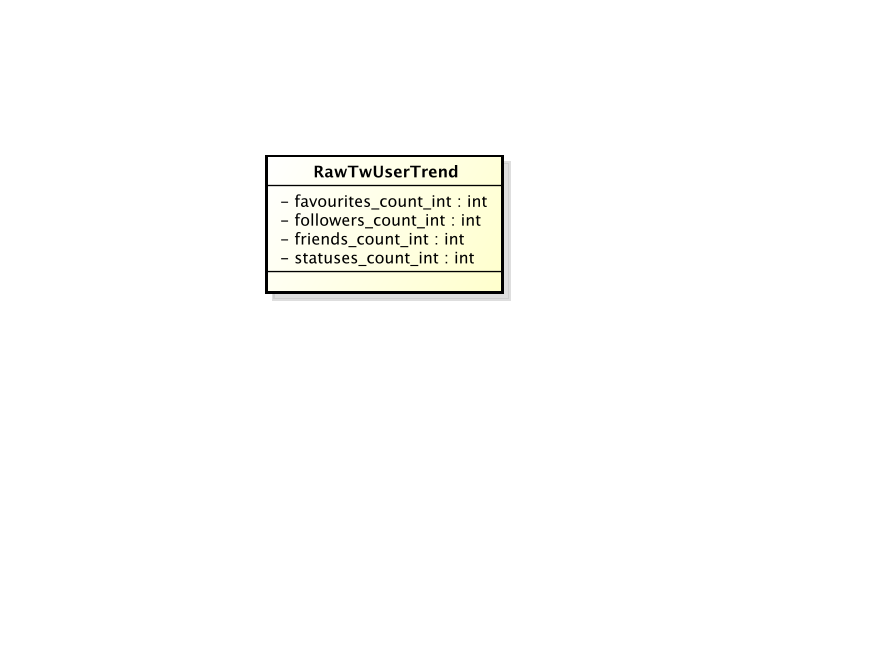
\includegraphics[scale=0.75]{./images/server/classes/db/raw_tw_user_trend.pdf}}
				\caption{Classe - server::db::raw\_data::tw::RawTwUserTrend}
			\end{figure}
			\begin{itemize}
				\item \textbf{Descrizione}: classe che definisce il modello dei dati del trend di un utente Twitter;
				\item \textbf{Utilizzo}: la classe viene utilizzata per memorizzare il numero di favoriti, di followers, di friends e statuses di un determinato utente Twitter. Come per tutti gli oggetti di tipo trend, vengono ricavati i dati fino a 3 giorni prima della creazione dell'oggetto;
				\item \textbf{Classi ereditate}: server::db::raw\_data::AbsTwRawData
				\item \textbf{Attributi}:
					\begin{itemize}
						\item \textcolor{forestgreen}{\texttt{+ favourites\_count\_int : int}}
						\begin{description}
							\item \textbf{Descrizione}: numero totale dei preferiti assegnati dall'utente.
						\end{description}
						\item \textcolor{forestgreen}{\texttt{+ followers\_count\_int : int}}
						\begin{description}
							\item \textbf{Descrizione}: numero dei followers di un utente Twitter.
						\end{description}
						\item \textcolor{forestgreen}{\texttt{+ friends\_count\_int : int}}
						\begin{description}
							\item \textbf{Descrizione}: numero dei following di un utente Twitter.
						\end{description}
						\item \textcolor{forestgreen}{\texttt{+ tweets\_count\_int : int}}
						\begin{description}
							\item \textbf{Descrizione}: numero di tweets di un utente Twitter.
						\end{description}
					\end{itemize}
				\item \textbf{Metodi}: N/A
			\end{itemize}
		% subparagraph server_db_raw_data_tw_rawigusertrend [end]


		\subparagraph{server::db::raw\_data::tw::RawTwUserTweet} % (fold)
		\label{subp:server_db_raw_data_tw_rawtwusertweet}
			\begin{figure}[htbp]
				\centering
				\centerline{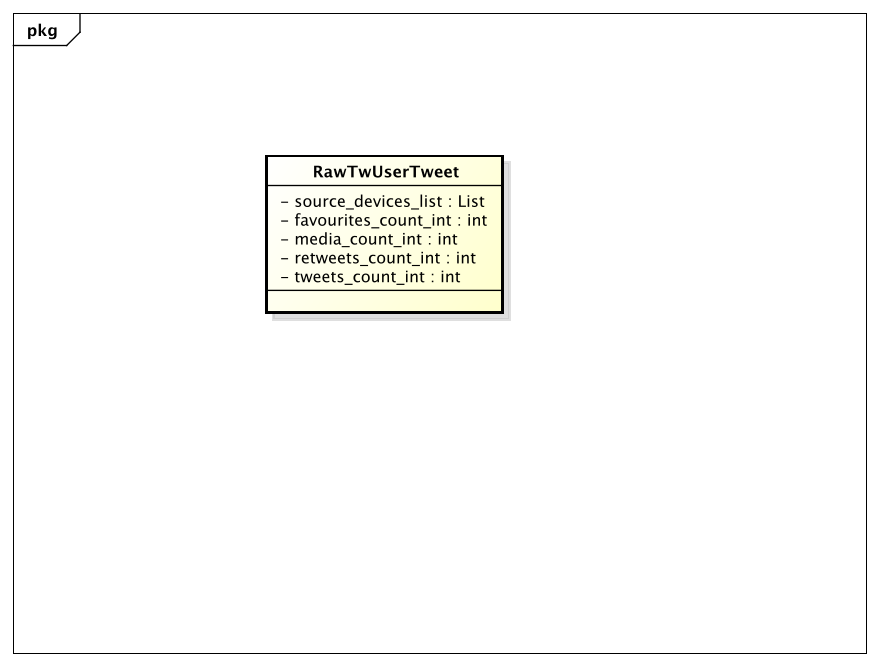
\includegraphics[scale=0.75]{./images/server/classes/db/raw_tw_user_tweet.pdf}}
				\caption{Classe - server::db::raw\_data::tw::RawTwUserTweet}
			\end{figure}
			\begin{itemize}
				\item \textbf{Descrizione}: classe che definisce il modello dei dati del trend dei tweet relativi ad un utente Twitter;
				\item \textbf{Utilizzo}: la classe viene utilizzata per fornire una descrizione dettagliata di un tweet creato da un utente specifico su Twitter;
				\item \textbf{Classi ereditate}: server::db::raw\_data::AbsRawData
				\item \textbf{Attributi}:
					\begin{itemize}
						\item \textcolor{forestgreen}{\texttt{+ source\_devices\_list : List}}
						\begin{description}
							\item \textbf{Descrizione}: lista composta da quantità e tipo dispositivi utilizzati in relazione ai tweet di un utente Twitter.
						\end{description}
						\item \textcolor{forestgreen}{\texttt{+ favourites\_count\_int : int}}
						\begin{description}
							\item \textbf{Descrizione}: totale dei preferiti aggiunti ai tweet di un utente.
						\end{description}
						\item \textcolor{forestgreen}{\texttt{+ retweets\_count\_int : int}}
						\begin{description}
							\item \textbf{Descrizione}: numero totale dei retweet ai tweets di utente Twitter.
						\end{description}
					\end{itemize}
				\item \textbf{Metodi}: N/A
			\end{itemize}
		% subparagraph server_db_raw_data_tw_rawtwusertweet [end]


		\subparagraph{server::db::raw\_data::tw::RawTwHashtag} % (fold)
		\label{subp:server_db_raw_data_tw_rawtwhashtag}
			\begin{itemize}
				\item \textbf{Descrizione}: classe che definisce il modello dei dati di un hashtag su Twitter;
				\item \textbf{Utilizzo}: la classe viene utilizzata per fornire una descrizione minimale di un hashtag su Twitter. Sebbene tale classe non presenti metodi o attributi, risulta molto utile per distinguere un hashtag Twitter da un'altra metrica effettuando un type checking;
				\item \textbf{Classi ereditate}: server::db::raw\_data::AbsTwRawData
				\item \textbf{Relazioni con altre classi}:
					\begin{itemize}
						\item server::db::raw\_data::tw::RawTwHashtagTweet
					\end{itemize}
				\item \textbf{Attributi}: N/A
				\item \textbf{Metodi}: N/A
			\end{itemize}
		% subparagraph server_db_raw_data_tw_rawtwhashtag [end]


		\subparagraph{server::db::raw\_data::tw::RawTwHashtagTweet} % (fold)
		\label{subp:server_db_raw_data_tw_rawtwhashtagtweet}
			\begin{figure}[htbp]
				\centering
				\centerline{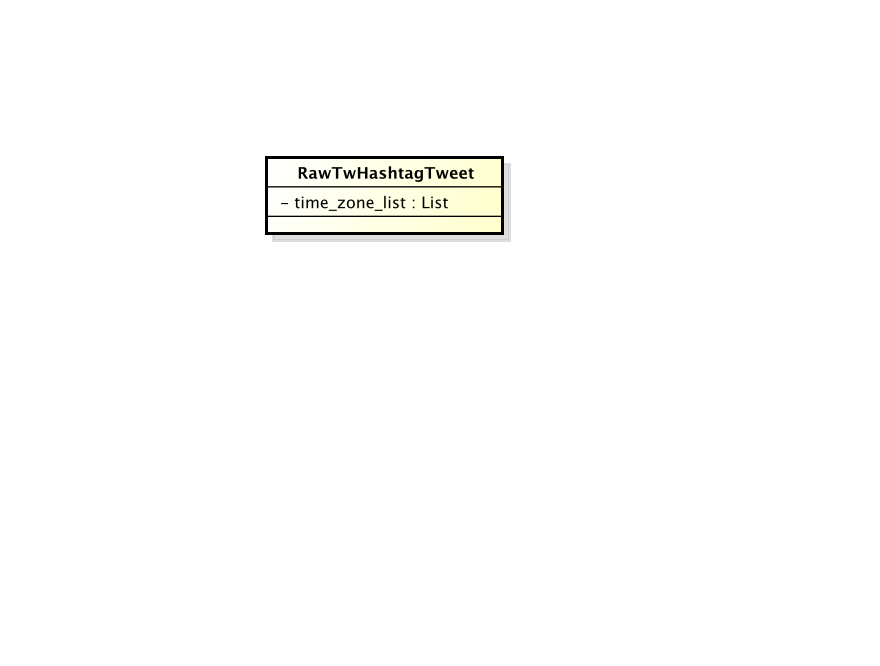
\includegraphics[scale=0.75]{./images/server/classes/db/raw_tw_hashtag_tweet.pdf}}
				\caption{Classe - server::db::raw\_data::tw::RawTwHashtagTweet}
			\end{figure}
			\begin{itemize}
				\item \textbf{Descrizione}: classe che definisce il modello dei dati del trend dei tweet relativi ad un hashtag Twitter;
				\item \textbf{Utilizzo}: la classe viene utilizzata per fornire una descrizione della locazione spaziale di un tweet relativo all'hashtag su Twitter. Come per tutti gli oggetti di tipo trend, vengono ricavati i dati fino a 3 giorni prima della creazione dell'oggetto;
				\item \textbf{Classi ereditate}: server::db::raw\_data::RawTwUserTweet
				\item \textbf{Attributi}:
					\begin{itemize}
						\item \textcolor{forestgreen}{\texttt{+ time\_zone\_list : List}}
						\begin{description}
							\item \textbf{Descrizione}: contiene informazioni sulle timezone ricavate dai vari tweet contenenti un determinato hashtag Twitter e dalle occorrenze delle stesse.
						\end{description}
						\item \textcolor{forestgreen}{\texttt{+ tweets\_count\_int : int}}
						\begin{description}
							\item \textbf{Descrizione}: totale dei tweet contenenti un determinato hashtag.
						\end{description}
					\end{itemize}
				\item \textbf{Metodi}: N/A
			\end{itemize}
		% subparagraph server_db_raw_data_tw_rawtwhashtagtweet [end]


		% subsubsection INSTAGRAM
		\subsubsection{server::db::raw\_data::ig} % (fold)
		\label{ssub:bdsm_app_server_db_raw_data_ig}
		\begin{figure}[htbp]
			\centering
			\centerline{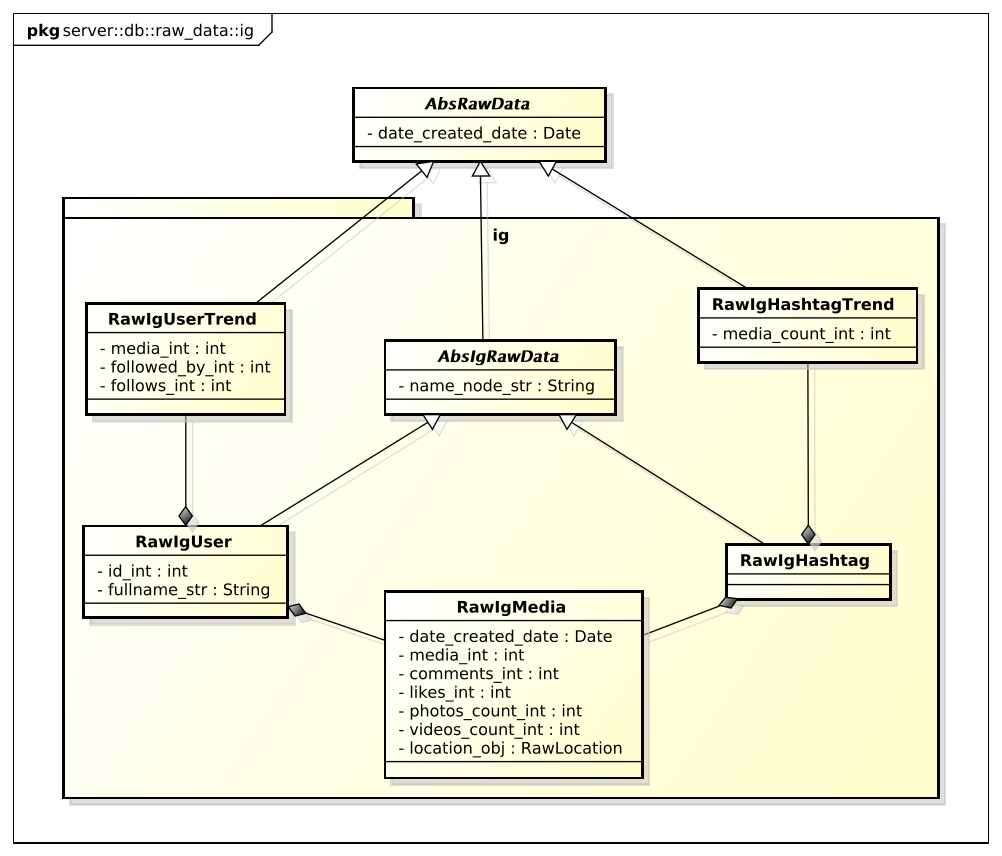
\includegraphics[scale=0.5]{./images/server/raw_data_ig.pdf}}
			\caption{Package - server::db::raw\_data::ig}
		\end{figure}

		\begin{itemize}
		  \item \textbf{Descrizione}: è il package contenente le classi che definiscono i modelli dei dati grezzi relativi a Instagram;
		  \item \textbf{Padre}: server::db::raw\_data
		  \item \textbf{Interazione con altri componenti}:
		  	\begin{itemize}
		  		\item server::db
				\end{itemize}
		\end{itemize}
		% subsubsection

		\paragraph{Classi} % (fold)


		\subparagraph{server::db::raw\_data::ig::AbsIgRawData} % (fold)
		\label{subp:server_db_raw_data_ig_absigrawdata}
			\begin{figure}[htbp]
				\centering
				\centerline{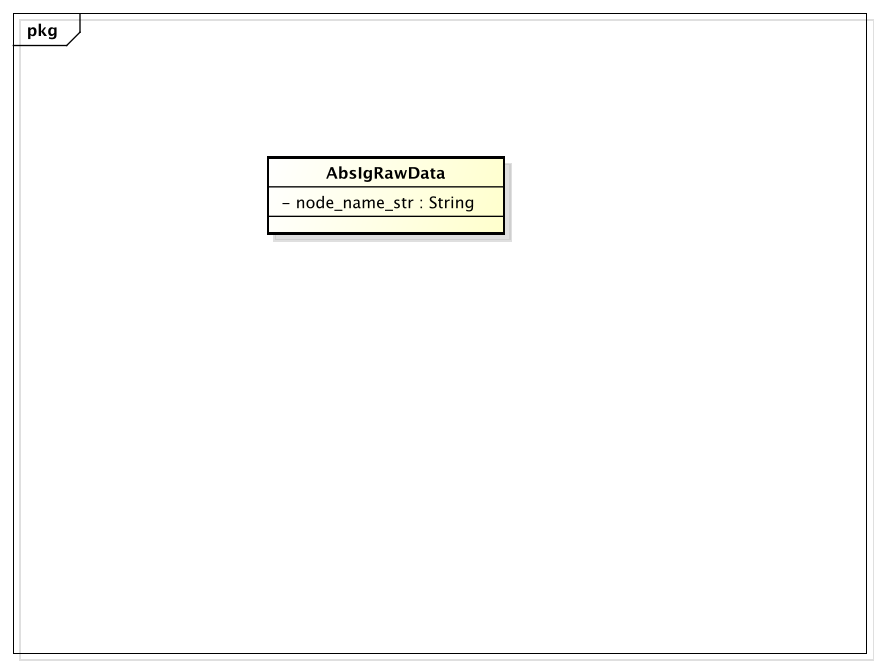
\includegraphics[scale=0.75]{./images/server/classes/db/abs_ig_raw_data.pdf}}
				\caption{Classe - server::db::raw\_data::ig::AbsIgRawData}
			\end{figure}
			\begin{itemize}
				\item \textbf{Descrizione}: classe astratta che definisce il modello dei dati grezzi relativi ad Instagram;
				\item \textbf{Utilizzo}: la classe contiene l'id fornito dall'utente il quale permette di identificare univocamente la risorsa nel social media;
				\item \textbf{Classi ereditate}: server::db::raw\_data::AbsRawData
				\item \textbf{Attributi}:
					\begin{itemize}
						\item \textcolor{forestgreen}{\texttt{+ node\_name\_str : String}}
						\begin{description}
							\item \textbf{Descrizione}: nome identificativo di un utente o di un hashtag Instagram.
						\end{description}
					\end{itemize}
				\item \textbf{Metodi}: N/A
			\end{itemize}
		% subparagraph server_db_raw_data_ig_absigrawdata [end]


		\subparagraph{server::db::raw\_data::ig::RawIgUser} % (fold)
		\label{subp:server_db_raw_data_ig_rawiguser}
			\begin{figure}[htbp]
				\centering
				\centerline{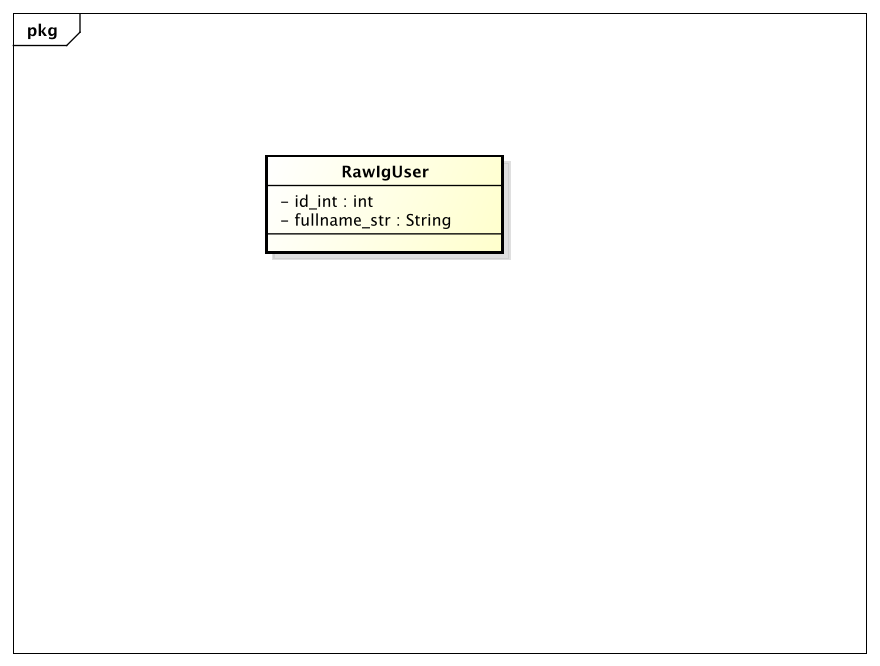
\includegraphics[scale=0.75]{./images/server/classes/db/raw_ig_user.pdf}}
				\caption{Classe - server::db::raw\_data::ig::RawIgUser}
			\end{figure}
			\begin{itemize}
				\item \textbf{Descrizione}: classe che definisce il modello dei dati di un utente Instagram;
				\item \textbf{Utilizzo}:  la classe viene utilizzata per memorizzare i dettagli di un utente Instagram;
				\item \textbf{Classi ereditate}: server::db::raw\_data::AbsIgRawData
				\item \textbf{Relazioni con altre classi}:
					\begin{itemize}
						\item server::db::raw\_data::ig::RawIgUserTrend
						\item server::db::raw\_data::ig::RawIgMedia
					\end{itemize}
				\item \textbf{Attributi}:
					\begin{itemize}
						\item \textcolor{forestgreen}{\texttt{+ id\_int : int}}
						\begin{description}
							\item \textbf{Descrizione}: numero identificativo di utente Instagram.
						\end{description}
						\item \textcolor{forestgreen}{\texttt{+ fullname\_str : String}}
						\begin{description}
							\item \textbf{Descrizione}: nome completo di utente Instagram.
						\end{description}
					\end{itemize}
				\item \textbf{Metodi}: N/A
			\end{itemize}
		% subparagraph server_db_raw_data_ig_rawiguser [end]


		\subparagraph{server::db::raw\_data::ig::RawIgUserTrend} % (fold)
		\label{subp:server_db_raw_data_ig_rawigusertrend}
			\begin{figure}[htbp]
				\centering
				\centerline{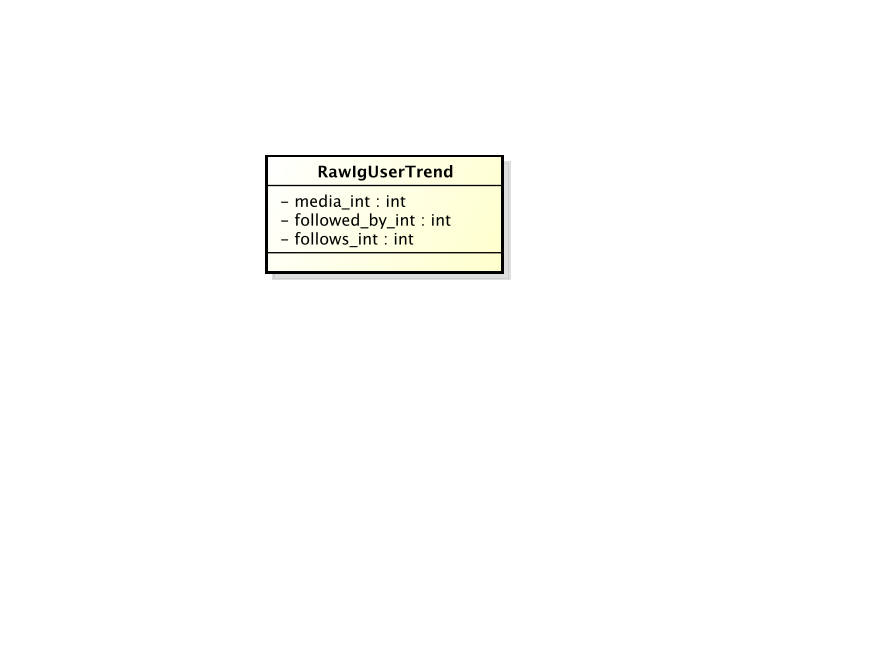
\includegraphics[scale=0.75]{./images/server/classes/db/raw_ig_user_trend.pdf}}
				\caption{Classe - server::db::raw\_data::ig::RawIgUserTrend}
			\end{figure}
			\begin{itemize}
				\item \textbf{Descrizione}: classe che definisce il modello dei dati del trend di un utente Instagram;
				\item \textbf{Utilizzo}: la classe viene utilizzata per memorizzare il numero di media, di followed e follows di una determinata persona. Come per tutti gli oggetti di tipo trend, vengono ricavati i dati fino a 3 giorni prima della creazione dell'oggetto;
				\item \textbf{Classi ereditate}: server::db::raw\_data::AbsRawData
				\item \textbf{Attributi}:
					\begin{itemize}
						\item \textcolor{forestgreen}{\texttt{+ media\_int : int}}
						\begin{description}
							\item \textbf{Descrizione}: numero di media caricati dall'utente su Instagram.
						\end{description}
						\item \textcolor{forestgreen}{\texttt{+ followed\_by\_int : int}}
						\begin{description}
							\item \textbf{Descrizione}: numero di followed dell'utente su Instagram.
						\end{description}
						\item \textcolor{forestgreen}{\texttt{+ follows\_int : int}}
						\begin{description}
							\item \textbf{Descrizione}: numero di following dell'utente su Instagram.
						\end{description}
					\end{itemize}
				\item \textbf{Metodi}: N/A
			\end{itemize}
		% subparagraph server_db_raw_data_ig_rawigusertrend [end]


		\subparagraph{server::db::raw\_data::ig::RawIgHashtag} % (fold)
		\label{subp:server_db_raw_data_ig_rawighashtag}
			\begin{itemize}
				\item \textbf{Descrizione}: classe che definisce il modello dei dati di un hashtag Instagram;
				\item \textbf{Utilizzo}: la classe viene utilizzata per fornire una descrizione minimale dell'hashtag su Instagram. Sebbene tale classe non fornisca metodi o campi dati, risulta molto utile per distinguere un hashtag Instagram da un'altra metrica tramite type checking;
				\item \textbf{Classi ereditate}: server::db::raw\_data::AbsIgRawData
				\item \textbf{Relazioni con altre classi}:
					\begin{itemize}
						\item server::db::raw\_data::ig::RawIgHashtagTrend
						\item server::db::raw\_data::ig::RawIgMedia
					\end{itemize}
				\item \textbf{Attributi}: N/A
				\item \textbf{Metodi}: N/A
			\end{itemize}
		% subparagraph server_db_raw_data_ig_rawighashtag [end]


		\subparagraph{server::db::raw\_data::ig::RawIgHashtagTrend} % (fold)
		\label{subp:server_db_raw_data_ig_rawighashtagtrend}
			\begin{figure}[htbp]
				\centering
				\centerline{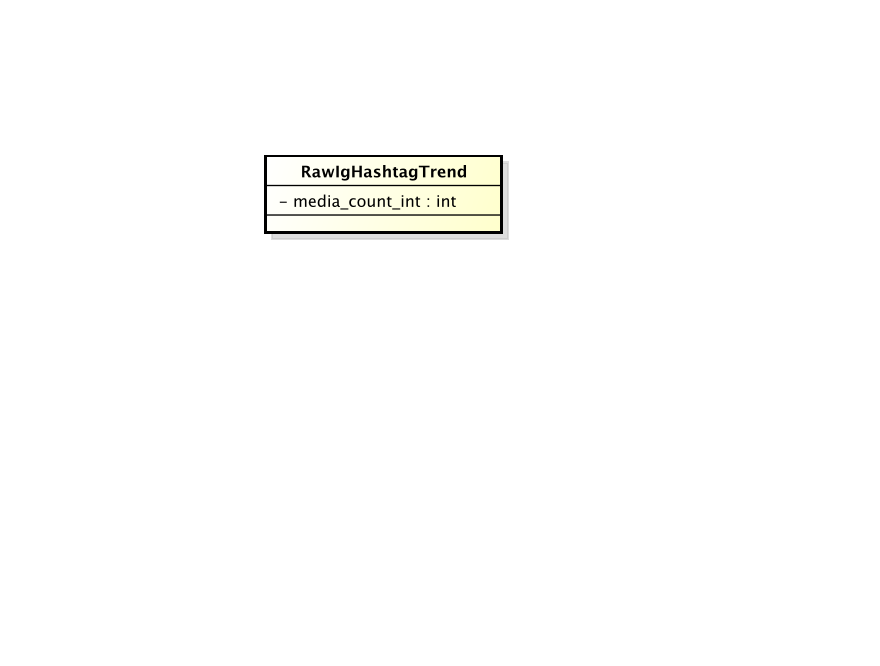
\includegraphics[scale=0.75]{./images/server/classes/db/raw_ig_hashtag_trend.pdf}}
				\caption{Classe - server::db::raw\_data::ig::RawIgHashtagTrend}
			\end{figure}
			\begin{itemize}
				\item \textbf{Descrizione}: classe che definisce il modello dei dati del trend di un hashtag Instagram;
				\item \textbf{Utilizzo}: la classe viene utilizzata per memorizzare il numero di media caricati di un determinato hashtag. Come per tutti gli oggetti di tipo trend, vengono ricavati i dati fino a 3 giorni prima della creazione dell'oggetto;
				\item \textbf{Classi ereditate}: server::db::raw\_data::AbsRawData
				\item \textbf{Attributi}:
					\begin{itemize}
						\item \textcolor{forestgreen}{\texttt{+ media\_count\_int : int}}
						\begin{description}
							\item \textbf{Descrizione}: numero totale di media relativi ad un hashtag su Instagram.
						\end{description}
					\end{itemize}
				\item \textbf{Metodi}: N/A
			\end{itemize}
		% subparagraph server_db_raw_data_ig_rawighashtagtrend [end]


		\subparagraph{server::db::raw\_data::ig::RawIgMedia} % (fold)
		\label{subp:server_db_raw_data_ig_rawigmedia}
			\begin{figure}[htbp]
				\centering
				\centerline{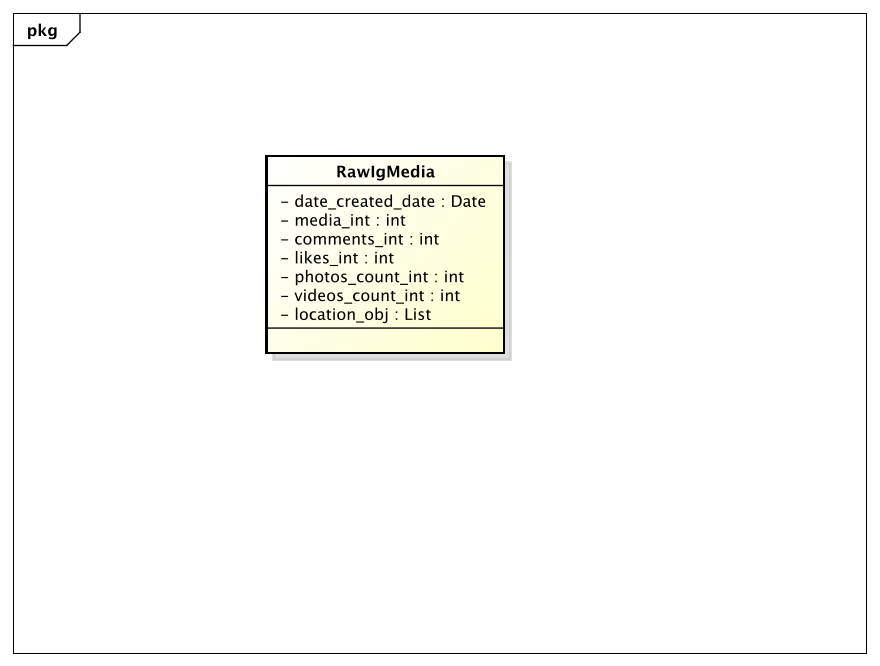
\includegraphics[scale=0.75]{./images/server/classes/db/raw_ig_media.pdf}}
				\caption{Classe - server::db::raw\_data::ig::RawIgMedia}
			\end{figure}
			\begin{itemize}
				\item \textbf{Descrizione}: classe che definisce il modello dei dati di un media relativo ad Instagram;
				\item \textbf{Utilizzo}: la classe viene utilizzata per fornire una descrizione dettagliata del trend dei media relativi ad un utente o un hashtag specifico su Instagram. Come per tutti gli oggetti di tipo trend, vengono ricavati i dati fino a 3 giorni prima della creazione dell'oggetto;
				\item \textbf{Classi ereditate}: server::db::raw\_data::AbsRawData
				\item \textbf{Attributi}:
					\begin{itemize}
						\item \textcolor{forestgreen}{\texttt{+ media\_int : int}}
						\begin{description}
							\item \textbf{Descrizione}: numero di media ricavati.
						\end{description}
						\item \textcolor{forestgreen}{\texttt{+ comments\_int : int}}
						\begin{description}
							\item \textbf{Descrizione}: numero totale dei commenti presenti in tutti i media ricavati.
						\end{description}
						\item \textcolor{forestgreen}{\texttt{+ likes\_int : int}}
						\begin{description}
							\item \textbf{Descrizione}: numero totale dei likes presenti in tutti i media ricavati.
						\end{description}
						\item \textcolor{forestgreen}{\texttt{+ photos\_count\_int : int}}
						\begin{description}
							\item \textbf{Descrizione}: numero totale di media di tipo foto.
						\end{description}
						\item \textcolor{forestgreen}{\texttt{+ videos\_count\_int : int}}
						\begin{description}
							\item \textbf{Descrizione}: numero totale di media di tipo video.
						\end{description}
						\item \textcolor{forestgreen}{\texttt{+ location\_obj : GeoPoint}}
						\begin{description}
							\item \textbf{Descrizione}: localizzazione tramite latitudine e longitudine di un media su Instagram.
						\end{description}
					\end{itemize}
				\item \textbf{Metodi}: N/A
			\end{itemize}
		% subparagraph server_db_raw_data_ig_rawigmedia [end]

\subsubsection{server::db::app\_data} % (fold)
\label{ssub:bdsm_app_server_app_data}


	\begin{figure}[htbp]
		\centering
		\centerline{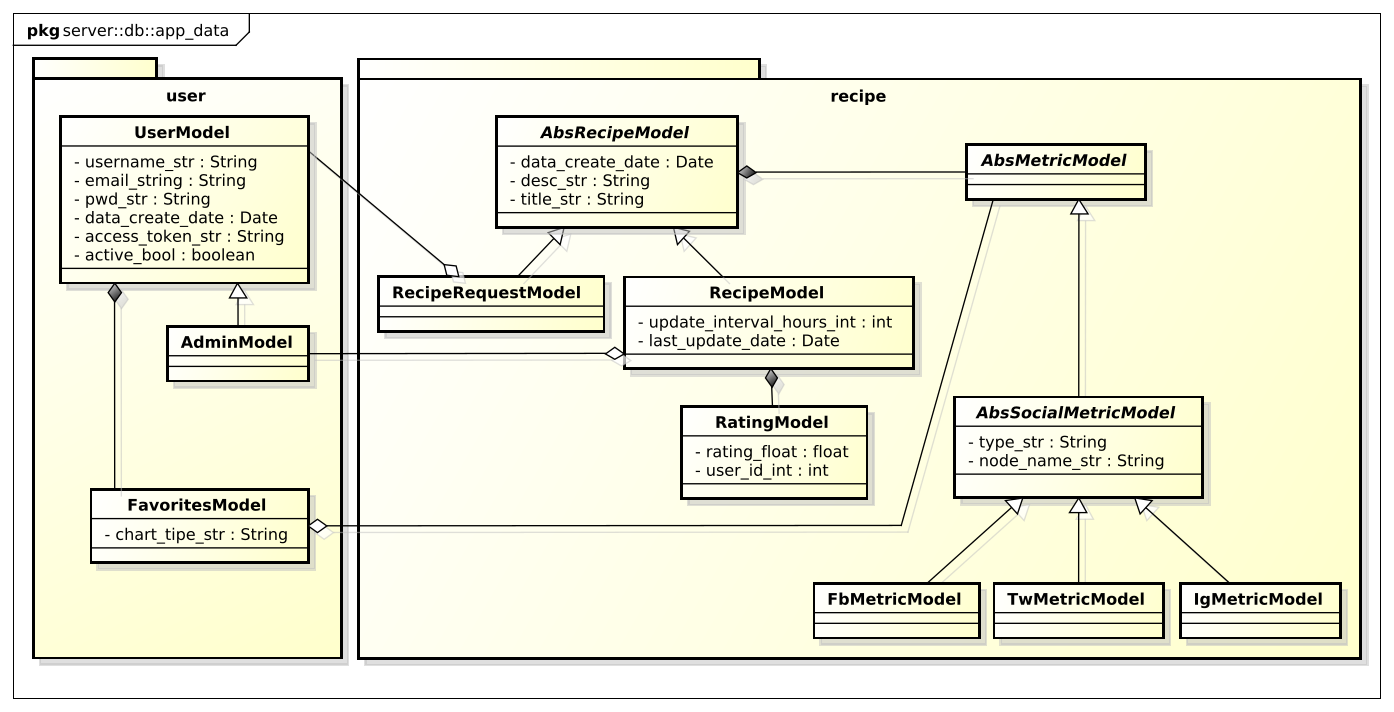
\includegraphics[scale=0.38]{./images/server/app_data.pdf}}
		\caption{Package - server::db::app\_data}
	\end{figure}


	\begin{itemize}
		\item \textbf{Descrizione}: è il package che contiene la definizione dei modelli degli utenti registrati e le loro preferenze. Contiene inoltre il modello delle Recipe che l'amministratore decide di creare;
		\item \textbf{Padre}: server::db
		\item \textbf{Package contenuti}
			\begin{itemize}
				\item server::db::app\_data::user
				\item server::db::app\_data::recipe
			\end{itemize}
	\end{itemize}
	% subsubsection bdsm_app_server_app_data [end]


\subsubsection{server::db::app\_data::user} % (fold)
\label{ssub:bdsm_app_server_app_data_user}

	\begin{itemize}
		\item \textbf{Descrizione}: è il package che contiene la definizione dei modelli degli utenti registrati e le loro preferenze;
		\item \textbf{Padre}: server::db::app\_data
		\item \textbf{Interazione con altri componenti}:
			\begin{itemize}
				\item server::db::app\_data::recipe
			\end{itemize}
	\end{itemize}
	% subsubsection bdsm_app_server_app_data_user [end]


	\paragraph{Classi} % (fold)

		\subparagraph{server::db::app\_data::user::UserModel} % (fold)
		\label{subp:server_db_app_data_user_user_model}
			\begin{figure}[htbp]
				\centering
				\centerline{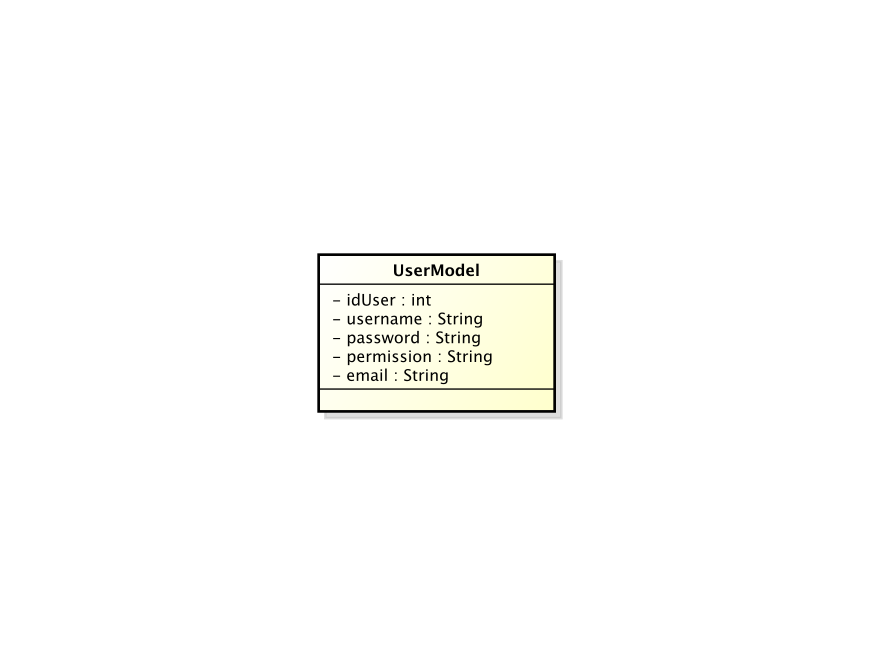
\includegraphics[scale=0.75]{./images/server/classes/db/user_model.pdf}}
				\caption{Classe - server::db::app\_data::user::UserModel}
			\end{figure}
			\begin{itemize}
				\item \textbf{Descrizione}: classe che definisce il modello dei dati degli utenti all'interno della base di dati;
				\item \textbf{Utilizzo}: la classe utilizzata per aggiungere, modificare o eliminare un utente dal database;
				\item \textbf{Relazioni con altre classi}:
					\begin{itemize}
						\item server::db::app\_data::user::FavouritesModel
						\item server::db:::app\_data::user::AdminModel
						\item server::db::app\_data::recipe::RecipeRequestModel
					\end{itemize}
				\item \textbf{Attributi}:
					\begin{itemize}
						\item \textcolor{forestgreen}{\texttt{+ username\_str : String}}
						\begin{description}
							\item \textbf{Descrizione}: lo username dell'utente.
						\end{description}
						\item \textcolor{forestgreen}{\texttt{+ email\_str : String}}
						\begin{description}
							\item \textbf{Descrizione}: l'email dell'utente.
						\end{description}
						\item \textcolor{forestgreen}{\texttt{+ pwd\_str : String}}
						\begin{description}
							\item \textbf{Descrizione}: la password dell'utente.
						\end{description}
						\item \textcolor{forestgreen}{\texttt{+ data\_created\_date : Date}}
						\begin{description}
							\item \textbf{Descrizione}: la data creazione account dell'utente.
						\end{description}
						\item \textcolor{forestgreen}{\texttt{+ access\_token\_str : String}}
						\begin{description}
							\item \textbf{Descrizione}: l'access token utilizzato per i servizi REST.
						\end{description}
						\item \textcolor{forestgreen}{\texttt{+ oauth\_token : String}}
						\begin{description}
							\item \textbf{Descrizione}: il token utilizzato per il processo di autenticazione dell'utente.
						\end{description}
						\item \textcolor{forestgreen}{\texttt{+ active\_bool : boolean}}
						\begin{description}
							\item \textbf{Descrizione}: valore che indica se l'utente attivo nel sistema.
						\end{description}
					\end{itemize}
				\item \textbf{Metodi}: N/A
			\end{itemize}
		% subparagraph server_db_app_data_user_user_model [end]


		\subparagraph{server::db::app\_data::user::AdminModel} % (fold)
		\label{subp:server_db_app_data_user_admin_model}
			\begin{itemize}
				\item \textbf{Descrizione}: classe che definisce il modello dei dati degli utenti amministratori all'interno della base di dati;
				\item \textbf{Utilizzo}: la classe specializza l'utente amministratore. Viene utilizzata esclusivamente per distinguere un amministratore da un utente normale tramite type checking;
				\item \textbf{Classi ereditate}: server::db::app\_data::user::UserModel;
				\item \textbf{Relazioni con altre classi}:
					\begin{itemize}
						\item server::db::app\_data::recipe::RecipeModel
					\end{itemize}
				\item \textbf{Attributi}: N/A
				\item \textbf{Metodi}: N/A
			\end{itemize}
		% subparagraph server_db_app_data_user_admin_model [end]


		\subparagraph{server::db::app\_data::user::FavouritesModel} % (fold)
		\label{subp:server_db_app_data_user_favorites}
			\begin{figure}[htbp]
				\centering
				\centerline{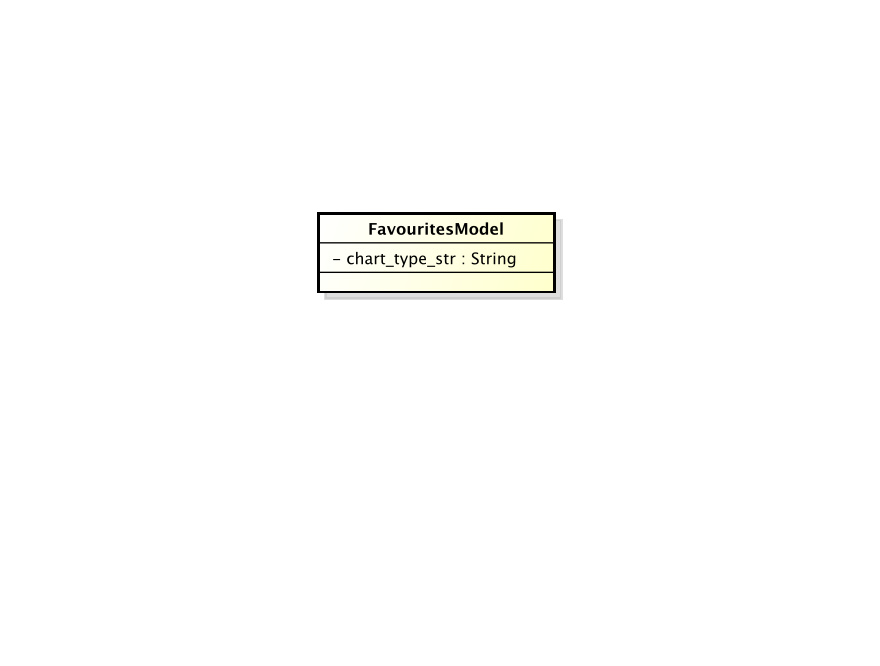
\includegraphics[scale=0.75]{./images/server/classes/db/favourites_model.pdf}}
				\caption{Classe - server::db::app\_data::user::FavouritesModel}
			\end{figure}
			\begin{itemize}
				\item \textbf{Descrizione}: classe che definisce il modello dei dati relativo ai preferiti dell'utente;
				\item \textbf{Utilizzo}: la classe viene utilizzata per memorizzare e ricavare le View preferite relative ad un utente.
				\item \textbf{Relazioni con altre classi}:
					\begin{itemize}
						\item server::db::app\_data::recipe::AbsMetricModel
					\end{itemize}
				\item \textbf{Attributi}:
					\begin{itemize}
						\item \textcolor{forestgreen}{\texttt{chart\_type\_str : String}}
						\begin{description}
							\item \textbf{Descrizione}: tipo di grafico scelto dall'utente e salvato nei preferiti.
						\end{description}
					\end{itemize}
				\item \textbf{Metodi}: N/A
			\end{itemize}
		% subparagraph server_db_app_data_user_favorites [end]


\subsubsection{server::db::app\_data::recipe} % (fold)
\label{ssub:bdsm_app_server_app_data_recipe}

	\begin{itemize}
		\item \textbf{Descrizione}: è il package che contiene la definizione dei modelli delle Recipe che l'amministratore decide di creare;
		\item \textbf{Padre}: server::db::app\_data
		\item \textbf{Interazione con altri componenti}:
			\begin{itemize}
				\item server::db::app\_data::user
			\end{itemize}
	\end{itemize}
	% subsubsection bdsm_app_server_app_data_recipe [end]


	\paragraph{Classi} % (fold)

		\subparagraph{server::db::app\_data::recipe::AbsRecipeModel} % (fold)
		\label{subp:server_db_app_data_recipe_absrecipemodel}
			\begin{figure}[htbp]
				\centering
				\centerline{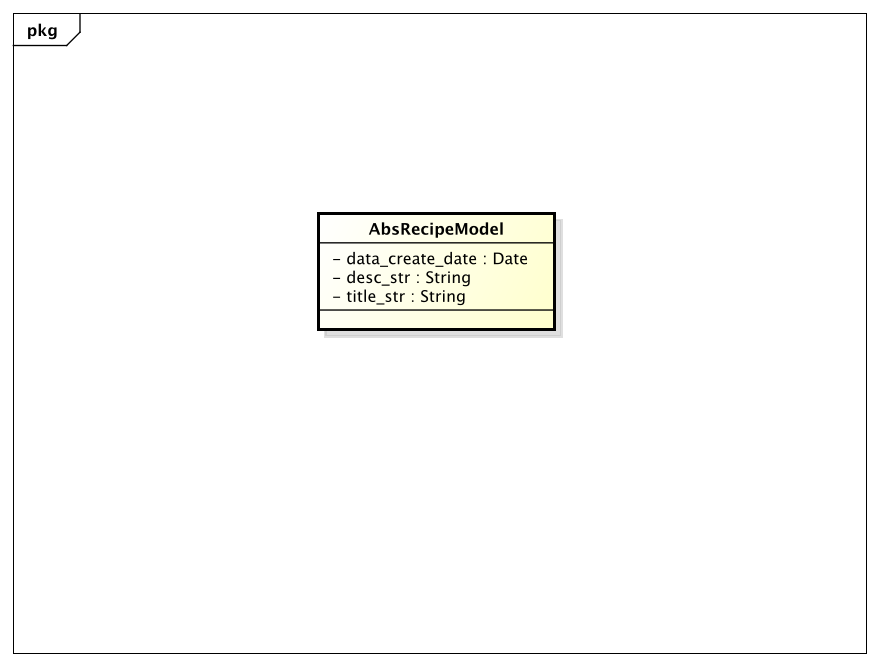
\includegraphics[scale=0.75]{./images/server/classes/db/abs_recipe_model.pdf}}
				\caption{Classe - server::db::app\_data::recipe::AbsRecipeModel}
			\end{figure}
			\begin{itemize}
				\item \textbf{Descrizione}: classe astratta che rappresenta un modello comune per Recipe e richiesta di aggiunta Recipe;
				\item \textbf{Utilizzo}: la classe mantiene l'estensibilità per eventuali nuovi tipi di Recipe;
				\item \textbf{Relazioni con altre classi}:
					\begin{itemize}
						\item server::db::app\_data::recipe::RecipeModel
						\item server::db::app\_data::recipe::RecipeRequestModel
						\item server::db::app\_data::recipe::AbsMetricModel
					\end{itemize}
				\item \textbf{Attributi}:
					\begin{itemize}
						\item \textcolor{forestgreen}{\texttt{data\_create\_date : Date}}
						\begin{description}
							\item \textbf{Descrizione}: data di creazione della Recipe.
						\end{description}
						\item \textcolor{forestgreen}{\texttt{desc\_str : String}}
						\begin{description}
							\item \textbf{Descrizione}: descrizione dettagliata dell Recipe.
						\end{description}
						\item \textcolor{forestgreen}{\texttt{title\_str : String}}
						\begin{description}
							\item \textbf{Descrizione}: titolo della Recipe.
						\end{description}
					\end{itemize}
				\item \textbf{Metodi}: N/A
			\end{itemize}
		% subparagraph server_db_app_data_recipe_absrecipemodel [end]


		\subparagraph{server::db::app\_data::recipe::RecipeRequestModel} % (fold)
		\label{subp:server_db_app_data_recipe_reciperequestmodel}
			\begin{itemize}
				\item \textbf{Descrizione}: classe che definisce il modello dei dati per la richiesta di aggiunta Recipe;
				\item \textbf{Utilizzo}: la classe specializza la richiesta identificandone l'utente tramite il rapporto parent-child delle classi di Google Datastore;
				\item \textbf{Classi ereditate}: server::db::app\_data::recipe::AbsRecipeModel
				\item \textbf{Attributi}: N/A
				\item \textbf{Metodi}: N/A
			\end{itemize}
		% subparagraph server_db_app_data_recipe_reciperequestmodel [end]


		\subparagraph{server::db::app\_data::recipe::RecipeModel} % (fold)
		\label{subp:server_db_app_data_recipe_recipemodel}
			\begin{figure}[htbp]
				\centering
				\centerline{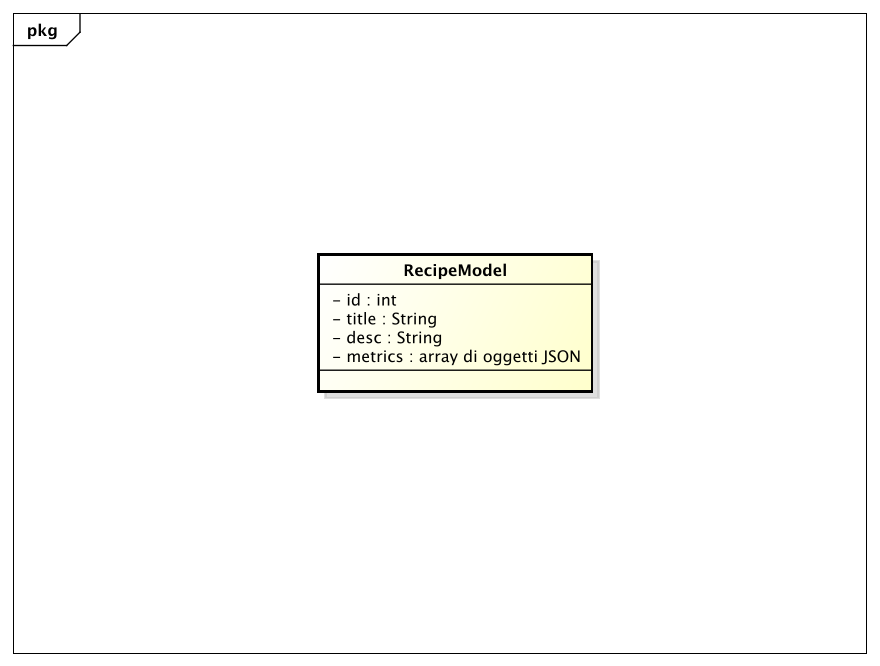
\includegraphics[scale=0.75]{./images/server/classes/db/recipe_model.pdf}}
				\caption{Classe - server::db::app\_data::recipe::RecipeModel}
			\end{figure}
			\begin{itemize}
				\item \textbf{Descrizione}: classe che definisce il modello dei dati relativo ad una Recipe;
				\item \textbf{Utilizzo}: la classe specializza la ricetta. Vengono forniti i campi dati per il possibile incremento temporale dei dati;
				\item \textbf{Classi ereditate}: server::db::app\_data::recipe::AbsRecipeModel
				\item \textbf{Relazioni con altre classi}:
					\begin{itemize}
						\item server::db::app\_data::recipe::RatingModel
					\end{itemize}
				\item \textbf{Attributi}:
					\begin{itemize}
						\item \textcolor{forestgreen}{\texttt{+ update\_interval\_hours\_int : int}}
						\begin{description}
							\item \textbf{Descrizione}: intervallo di tempo per la schedulazione dell'update della Recipe.
						\end{description}
						\item \textcolor{forestgreen}{\texttt{+ last\_update\_date : Date}}
						\begin{description}
							\item \textbf{Descrizione}: data dell'ultimo processo di update Recipe.
						\end{description}
					\end{itemize}
				\item \textbf{Metodi}: N/A
			\end{itemize}
		% subparagraph server_db_app_data_recipe_recipemodel [end]

		\subparagraph{server::db::app\_data::recipe::RatingModel} % (fold)
		\label{subp:server_db_app_data_recipe_recipemodel}
			\begin{figure}[htbp]
				\centering
				\centerline{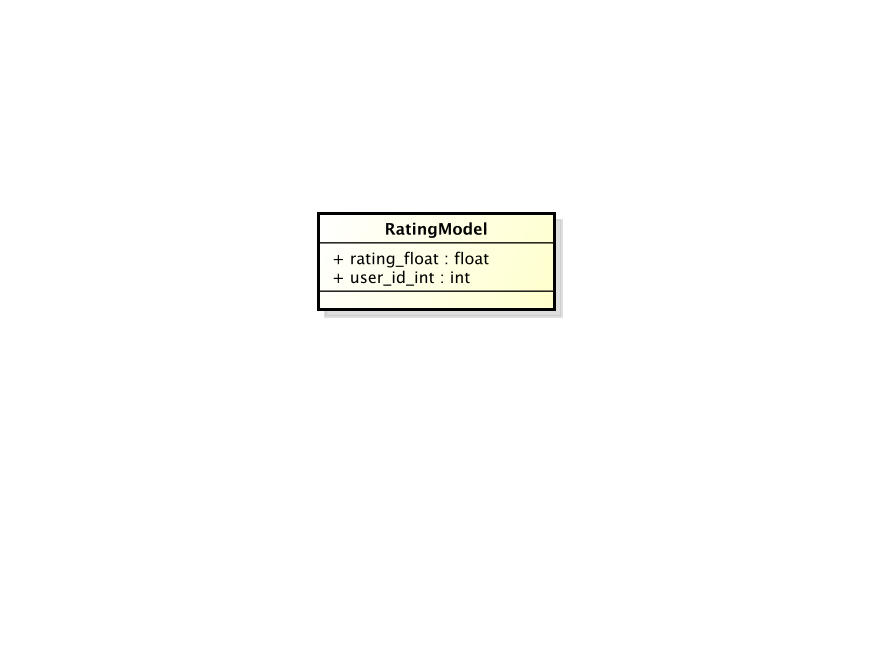
\includegraphics[scale=0.75]{./images/server/classes/db/rating_model.pdf}}
				\caption{Classe - server::db::app\_data::recipe::RatingModel}
			\end{figure}
			\begin{itemize}
				\item \textbf{Descrizione}: classe che rappresenta il modello del rating di una Recipe;
				\item \textbf{Utilizzo}: viene utilizzata per risalire al voto di ogni utente per una determinata Recipe;
				\item \textbf{Attributi}:
					\begin{itemize}
						\item \textcolor{forestgreen}{\texttt{+ rating\_float : float}}
						\begin{description}
							\item \textbf{Descrizione}: punteggio gradimento relativo alla Recipe.
						\end{description}
						\item \textcolor{forestgreen}{\texttt{+ user\_id\_int : int}}
					\end{itemize}
					\begin{description}
							\item \textbf{Descrizione}: identificativo dell'utente votante.
						\end{description}
				\item \textbf{Metodi}: N/A
			\end{itemize}
		% subparagraph server_db_app_data_recipe_recipemodel [end]


		\subparagraph{server::db::app\_data::recipe::AbsMetricModel} % (fold)
		\label{subp:server_db_app_data_recipe_absmetricmodel}
			\begin{itemize}
				\item \textbf{Descrizione}: classe che definisce il modello dei dati di una metrica contenuta in una Ricetta;
				\item \textbf{Utilizzo}: la classe rappresenta il modello dei dati di una metrica generale;
				\item \textbf{Relazioni con altre classi}:
					\begin{itemize}
						\item server::db::app\_data::recipe::AbsSocialMetricModel
					\end{itemize}
				\item \textbf{Attributi}: N/A
				\item \textbf{Metodi}: N/A
			\end{itemize}
		% subparagraph server_db_app_data_recipe_absmetricmodel [end]


		\subparagraph{server::db::app\_data::recipe::AbsSocialMetricModel} % (fold)
		\label{subp:server_db_app_data_recipe_abssocialmetricmodel}
			\begin{figure}[htbp]
				\centering
				\centerline{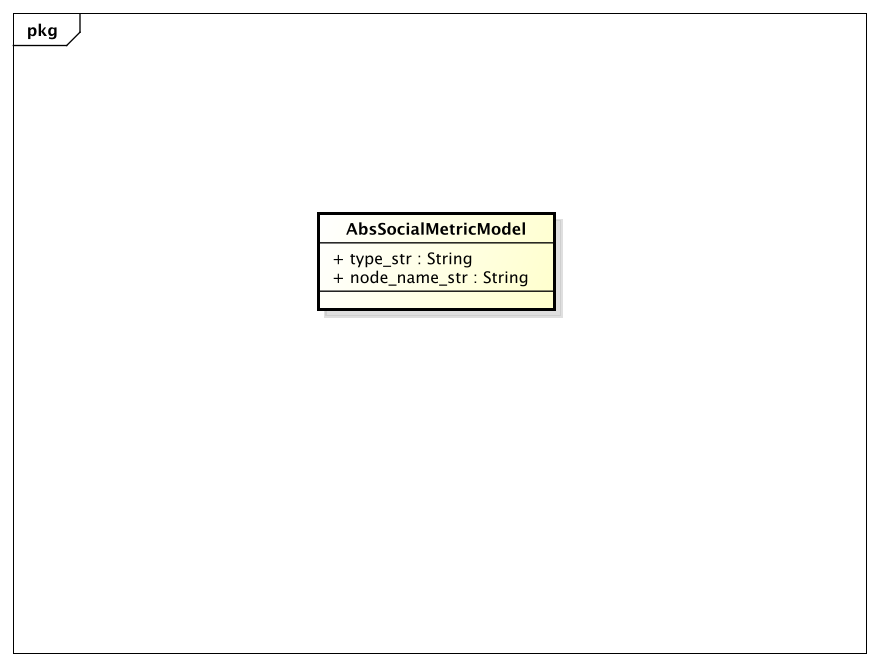
\includegraphics[scale=0.75]{./images/server/classes/db/abs_social_metric_model.pdf}}
				\caption{Classe - server::db::app\_data::recipe::AbsSocialMetricModel}
			\end{figure}
			\begin{itemize}
				\item \textbf{Descrizione}: classe che definisce il modello dei dati delle metriche relative ai social media;
				\item \textbf{Utilizzo}: la classe rappresenta il modello di una metrica relativa ad un social network fornendo il tipo di metrica e il suo identificativo;
				\item \textbf{Classi ereditate}: server::db::app\_data::recipe::AbsMetricModel
				\item \textbf{Relazioni con altre classi}:
					\begin{itemize}
						\item server::db::app\_data::recipe::FbMetricModel
						\item server::db::app\_data::recipe::IgMetricModel
						\item server::db::app\_data::recipe::TwMetricModel
					\end{itemize}
				\item \textbf{Attributi}:
					\begin{itemize}
						\item \textcolor{forestgreen}{\texttt{+ type\_str : String}}
						\begin{description}
							\item \textbf{Descrizione}: tipo della metrica (pagina, evento, hashtag).
						\end{description}
						\item \textcolor{forestgreen}{\texttt{+ node\_name\_str : String}}
						\begin{description}
							\item \textbf{Descrizione}: nome identificativo della metrica.
						\end{description}
					\end{itemize}
				\item \textbf{Metodi}: N/A
			\end{itemize}
		% subparagraph server_db_app_data_recipe_abssocialmetricmodel [end]


		\subparagraph{server::db::app\_data::recipe::FbMetricModel} % (fold)
		\label{subp:server_db_app_data_recipe_fbmetricmodel}
			\begin{itemize}
				\item \textbf{Descrizione}: classe che definisce il modello dei dati delle metriche relative a Facebook;
				\item \textbf{Utilizzo}: viene utilizzata esclusivamente per offrire una distinzione di tipo per le metriche relative a Facebook rispetto ai restanti social network;
				\item \textbf{Classi ereditate}: server::db::app\_data::recipe::AbsSocialMetricModel;
				\item \textbf{Attributi}: N/A
				\item \textbf{Metodi}: N/A
			\end{itemize}
		% subparagraph server_db_app_data_recipe_fbmetricmodel [end]


		\subparagraph{server::db::app\_data::recipe::IgMetricModel} % (fold)
		\label{subp:server_db_app_data_recipe_igmetricmodel}
			\begin{itemize}
				\item \textbf{Descrizione}: classe che definisce il modello dei dati delle metriche relative a Instagram;
				\item \textbf{Utilizzo}: viene utilizzata esclusivamente per offrire una distinzione di tipo per le metriche relative a Instagram rispetto ai restanti social network;
				\item \textbf{Classi ereditate}: server::db::app\_data::recipe::AbsSocialMetricModel;
				\item \textbf{Attributi}: N/A
				\item \textbf{Metodi}: N/A
			\end{itemize}
		% subparagraph server_db_app_data_recipe_igmetricmodel [end]


		\subparagraph{server::db::app\_data::recipe::TwMetricModel} % (fold)
		\label{subp:server_db_app_data_recipe_twmetricmodel}
			\begin{itemize}
				\item \textbf{Descrizione}: classe che definisce il modello dei dati delle metriche relative a Twitter;
				\item \textbf{Utilizzo}: viene utilizzata esclusivamente per offrire una distinzione di tipo per le metriche relative a Twitter rispetto ai restanti social network;
				\item \textbf{Classi ereditate}: server::db::app\_data::recipe::AbsSocialMetricModel;
				\item \textbf{Attributi}: N/A
				\item \textbf{Metodi}: N/A
			\end{itemize}
		% subparagraph server_db_app_data_recipe_twmetricmodel [end]
 \clearpage \newpage
  % END PACKAGE DB

  % PACKAGE PROCESSOR
  % =================================================================================================
% File:			server_tier/processor.tex
% Description:	Definisce la sezione relativa al back-end dell'applicazione
% Created:		2015-04-07
% Author:		Cusinato Giacomo
% Email:		cusinato.giacomo@mashup-unipd.it
% =================================================================================================
% Modification History:
% Version		Modifier Date		Change											Author
% 0.0.1
% =================================================================================================

% CONTENUTO DEL CAPITOLO


\subsubsection{bdsm\_app::server::processor} % (fold)
\label{ssub:bdsm_app_server_processor}
[TO DO] (diagramma) \newline \newline

\begin{itemize}
  \item \textbf{Descrizione}: [TO DO];
  \item \textbf{Padre}: [TO DO] (qualora presente);
  \item \textbf{Package contenuti}: [TO DO] (qualora presente);
  \item \textbf{Interazione con altri componenti}: [TO DO];
\end{itemize}
% subsubsection
 \clearpage \newpage
  % END PACKAGE PROCESSOR

  % PACKAGE MINER
  % =================================================================================================
% File:			server_tier/miner.tex
% Description:	Definisce la sezione relativa al back-end dell'applicazione
% Created:		2015-04-07
% Author:		Cusinato Giacomo
% Email:		cusinato.giacomo@mashup-unipd.it
% =================================================================================================
% Modification History:
% Version		Modifier Date		Change											Author
% 0.0.1
% =================================================================================================

% CONTENUTO DEL CAPITOLO


\subsubsection{bdsm\_app::server::miner} % (fold)
\label{ssub:bdsm_app_server_miner}
[TO DO] (diagramma) \newline \newline

\begin{itemize}
  \item \textbf{Descrizione}: è il package che contiene tutte le classi con i metodi per prelevare i dati dai social network e per salvarli nel database;
  \item \textbf{Padre}: server;
  \item \textbf{Package contenuti}:
  	\begin{itemize}
  		\item fb;
  		\item ig;
  		\item tw;
  	\end{itemize}
  \item \textbf{Interazione con altri componenti}:
  	\begin{itemize}
  		\item server::processor
  		\item server::database
  	\end{itemize}
\end{itemize}

\paragraph{Classi} % (fold)
		\subparagraph{server::miner::MinerScheduler} % (fold)
		\label{subp:server_miner_MinerScheduler}
			\begin{itemize}
				\item \textbf{Descrizione}:
				\item \textbf{Utilizzo}: 
				\item \textbf{Relazioni con altre classi}:
					\begin{itemize}
						\item 
					\end{itemize}
			\end{itemize}
		% subparagraph server_miner_MinerScheduler
		
		\subparagraph{server::miner::AbsCounter} % (fold)
		\label{subp:server_miner_AbsCounter}
			\begin{itemize}
				\item \textbf{Descrizione}: 
				\item \textbf{Utilizzo}: 
				\item \textbf{Relazioni con altre classi}:
					\begin{itemize}
						\item 
					\end{itemize}
			\end{itemize}
		% subparagraph server_miner_AbsCounter
		
		\subparagraph{server::miner::AbsFetcher} % (fold)
		\label{subp:server_miner_AbsFetcher}
			\begin{itemize}
				\item \textbf{Descrizione}: 
				\item \textbf{Utilizzo}: 
				\item \textbf{Relazioni con altre classi}:
					\begin{itemize}
						\item 
					\end{itemize}
			\end{itemize}
		% subparagraph server_miner_AbsFetcher
		
\subsubsection{bdsm\_app::server::miner::fb} % (fold)
\label{ssub:bdsm_app_server_miner_fb}
[TO DO] (diagramma) \newline \newline

\begin{itemize}
  \item \textbf{Descrizione}:
  \item \textbf{Padre}:
  \item \textbf{Package contenuti}:
  	\begin{itemize}
  		\item
  	\end{itemize}
  \item \textbf{Interazione con altri componenti}:
  	\begin{itemize}
  		\item  	
  	\end{itemize}
\end{itemize}	

	\paragraph{Classi} % (fold)
		\subparagraph{server::miner::fb::AbsFbFetcher} % (fold)
		\label{subp:server_miner_fb_AbsFbFetcher}
			\begin{itemize}
				\item \textbf{Descrizione}:
				\item \textbf{Utilizzo}: 
				\item \textbf{Relazioni con altre classi}:
					\begin{itemize}
						\item 
					\end{itemize}
			\end{itemize}
	% subparagraph server_miner_fb_AbsFbFetcher
	
		\subparagraph{server::miner::fb::FbPageFetcher} % (fold)
		\label{subp:server_miner_fb_FbPageFetcher}
			\begin{itemize}
				\item \textbf{Descrizione}:
				\item \textbf{Utilizzo}: 
				\item \textbf{Relazioni con altre classi}:
					\begin{itemize}
						\item 
					\end{itemize}
			\end{itemize}
	% subparagraph server_miner_fb_FbPageFetcher
	
		\subparagraph{server::miner::fb::FbEventFetcher} % (fold)
		\label{subp:server_miner_fb_FbEventFetcher}
			\begin{itemize}
				\item \textbf{Descrizione}:
				\item \textbf{Utilizzo}: 
				\item \textbf{Relazioni con altre classi}:
					\begin{itemize}
						\item 
					\end{itemize}
			\end{itemize}
	% subparagraph server_miner_fb_FbEventFetcher
	
		\subparagraph{server::miner::fb::AbsFbCounter} % (fold)
		\label{subp:server_miner_fb_AbsFbCounter}
			\begin{itemize}
				\item \textbf{Descrizione}:
				\item \textbf{Utilizzo}: 
				\item \textbf{Relazioni con altre classi}:
					\begin{itemize}
						\item 
					\end{itemize}
			\end{itemize}
	% subparagraph server_miner_fb_AbsFbCounter
	
		\subparagraph{server::miner::fb::AttendingCounter} % (fold)
		\label{subp:server_miner_fb_AttendingCounter}
			\begin{itemize}
				\item \textbf{Descrizione}:
				\item \textbf{Utilizzo}: 
				\item \textbf{Relazioni con altre classi}:
					\begin{itemize}
						\item 
					\end{itemize}
			\end{itemize}
	% subparagraph server_miner_fb_AttendingCounter
	
		\subparagraph{server::miner::fb::MaybeCounter} % (fold)
		\label{subp:server_miner_fb_MaybeCounter}
			\begin{itemize}
				\item \textbf{Descrizione}:
				\item \textbf{Utilizzo}: 
				\item \textbf{Relazioni con altre classi}:
					\begin{itemize}
						\item 
					\end{itemize}
			\end{itemize}
	% subparagraph server_miner_fb_MaybeCounter
	
	\subparagraph{server::miner::fb::InvitedCounter} % (fold)
		\label{subp:server_miner_fb_InvitedCunter}
			\begin{itemize}
				\item \textbf{Descrizione}:
				\item \textbf{Utilizzo}: 
				\item \textbf{Relazioni con altre classi}:
					\begin{itemize}
						\item 
					\end{itemize}
			\end{itemize}
	% subparagraph server_miner_fb_InvitedCounter

	\subparagraph{server::miner::fb::RefusedCounter} % (fold)
		\label{subp:server_miner_fb_RefusedCounter}
			\begin{itemize}
				\item \textbf{Descrizione}:
				\item \textbf{Utilizzo}: 
				\item \textbf{Relazioni con altre classi}:
					\begin{itemize}
						\item 
					\end{itemize}
			\end{itemize}
	% subparagraph server_miner_fb_RefusedCounter
	
	\subparagraph{server::miner::fb::PostCounter} % (fold)
		\label{subp:server_miner_fb_PostCounter}
			\begin{itemize}
				\item \textbf{Descrizione}:
				\item \textbf{Utilizzo}: 
				\item \textbf{Relazioni con altre classi}:
					\begin{itemize}
						\item 
					\end{itemize}
			\end{itemize}
	% subparagraph server_miner_fb_PostCounter
	
	\subparagraph{server::miner::fb::CommentCounter} % (fold)
		\label{subp:server_miner_fb_CommentCounter}
			\begin{itemize}
				\item \textbf{Descrizione}:
				\item \textbf{Utilizzo}: 
				\item \textbf{Relazioni con altre classi}:
					\begin{itemize}
						\item 
					\end{itemize}
			\end{itemize}
	% subparagraph server_miner_fb_CommentCounter
	
	\subparagraph{server::miner::fb::LikeCounter} % (fold)
		\label{subp:server_miner_fb_LikeCounter}
			\begin{itemize}
				\item \textbf{Descrizione}:
				\item \textbf{Utilizzo}: 
				\item \textbf{Relazioni con altre classi}:
					\begin{itemize}
						\item 
					\end{itemize}
			\end{itemize}
	% subparagraph server_miner_fb_LikeCounter

\subsubsection{bdsm\_app::server::miner::tw} % (fold)
\label{ssub:bdsm_app_server_miner_tw}
[TO DO] (diagramma) \newline \newline

\begin{itemize}
  \item \textbf{Descrizione}:
  \item \textbf{Padre}:
  \item \textbf{Package contenuti}:
  	\begin{itemize}
  		\item
  	\end{itemize}
  \item \textbf{Interazione con altri componenti}:
  	\begin{itemize}
  		\item  	
  	\end{itemize}
\end{itemize}	

	\paragraph{Classi} % (fold)
	\subparagraph{server::miner::tw::AbsTwFetcher} % (fold)
		\label{subp:server_miner_tw_AbsTwFetcher}
			\begin{itemize}
				\item \textbf{Descrizione}:
				\item \textbf{Utilizzo}: 
				\item \textbf{Relazioni con altre classi}:
					\begin{itemize}
						\item 
					\end{itemize}
			\end{itemize}
		% subparagraph server_miner_tw_AbsTwFetcher
		
	\subparagraph{server::miner::tw::TwHashtagFetcher} % (fold)
		\label{subp:server_miner_tw_TwHashtagFetcher}
			\begin{itemize}
				\item \textbf{Descrizione}:
				\item \textbf{Utilizzo}: 
				\item \textbf{Relazioni con altre classi}:
					\begin{itemize}
						\item 
					\end{itemize}
			\end{itemize}
		% subparagraph server_miner_tw_TwHashtagFetcher
		
	\subparagraph{server::miner::tw::TwUserFetcher} % (fold)
		\label{subp:server_miner_tw_TwUserFetcher}
			\begin{itemize}
				\item \textbf{Descrizione}:
				\item \textbf{Utilizzo}: 
				\item \textbf{Relazioni con altre classi}:
					\begin{itemize}
						\item 
					\end{itemize}
			\end{itemize}
		% subparagraph server_miner_tw_TwUserFetcher
		
	\subparagraph{server::miner::tw::AbsTwCounter} % (fold)
		\label{subp:server_miner_tw_AbsTwCounter}
			\begin{itemize}
				\item \textbf{Descrizione}:
				\item \textbf{Utilizzo}: 
				\item \textbf{Relazioni con altre classi}:
					\begin{itemize}
						\item 
					\end{itemize}
			\end{itemize}
		% subparagraph server_miner_tw_AbsTwCounter
		
	\subparagraph{server::miner::tw::UserTweetCounter} % (fold)
		\label{subp:server_miner_tw_UserTweetCounter}
			\begin{itemize}
				\item \textbf{Descrizione}:
				\item \textbf{Utilizzo}: 
				\item \textbf{Relazioni con altre classi}:
					\begin{itemize}
						\item 
					\end{itemize}
			\end{itemize}
		% subparagraph server_miner_tw_UserTweetCounter
		
		
	\subparagraph{server::miner::tw::HashtagTweetCounter} % (fold)
		\label{subp:server_miner_tw_HashtagTweetCounter}
			\begin{itemize}
				\item \textbf{Descrizione}:
				\item \textbf{Utilizzo}: 
				\item \textbf{Relazioni con altre classi}:
					\begin{itemize}
						\item 
					\end{itemize}
			\end{itemize}
		% subparagraph server_miner_tw_HashtagTweetCounter

\subsubsection{bdsm\_app::server::miner::ig} % (fold)
\label{ssub:bdsm_app_server_miner_ig}
[TO DO] (diagramma) \newline \newline

\begin{itemize}
  \item \textbf{Descrizione}:
  \item \textbf{Padre}:
  \item \textbf{Package contenuti}:
  	\begin{itemize}
  		\item
  	\end{itemize}
  \item \textbf{Interazione con altri componenti}:
  	\begin{itemize}
  		\item  	
  	\end{itemize}
\end{itemize}	

	\paragraph{Classi} % (fold)
	\subparagraph{server::miner::ig::AbsIgFetcher} % (fold)
		\label{subp:server_miner_tw_AbsIgFetcher}
			\begin{itemize}
				\item \textbf{Descrizione}:
				\item \textbf{Utilizzo}: 
				\item \textbf{Relazioni con altre classi}:
					\begin{itemize}
						\item 
					\end{itemize}
			\end{itemize}
		% subparagraph server_miner_tw_AbsIgFetcher		

	\subparagraph{server::miner::ig::IgUserFetcher} % (fold)
		\label{subp:server_miner_tw_IgUserFetcher}
			\begin{itemize}
				\item \textbf{Descrizione}:
				\item \textbf{Utilizzo}: 
				\item \textbf{Relazioni con altre classi}:
					\begin{itemize}
						\item 
					\end{itemize}
			\end{itemize}
		% subparagraph server_miner_tw_IgUserFetcher		
		
	\subparagraph{server::miner::ig::IgHashtagFetcher} % (fold)
		\label{subp:server_miner_tw_IgHashtagFetcher}
			\begin{itemize}
				\item \textbf{Descrizione}:
				\item \textbf{Utilizzo}: 
				\item \textbf{Relazioni con altre classi}:
					\begin{itemize}
						\item 
					\end{itemize}
			\end{itemize}
		% subparagraph server_miner_tw_IgHashtagFetcher		
		
	\subparagraph{server::miner::ig::AbsIgCounter} % (fold)
		\label{subp:server_miner_tw_AbsIgCounter}
			\begin{itemize}
				\item \textbf{Descrizione}:
				\item \textbf{Utilizzo}: 
				\item \textbf{Relazioni con altre classi}:
					\begin{itemize}
						\item 
					\end{itemize}
			\end{itemize}
		% subparagraph server_miner_tw_AbsIgCounter		
		
		
	\subparagraph{server::miner::ig::MediaCounter} % (fold)
		\label{subp:server_miner_tw_MediaCounter}
			\begin{itemize}
				\item \textbf{Descrizione}:
				\item \textbf{Utilizzo}: 
				\item \textbf{Relazioni con altre classi}:
					\begin{itemize}
						\item 
					\end{itemize}
			\end{itemize}
		% subparagraph server_miner_tw_MediaCounter		

		
% subsubsection
 \clearpage \newpage
  % END PACKAGE MINER

  % PACKAGE ENDPOINTS
  % =================================================================================================
% File:			server_tier/endpoints.tex
% Description:	Definisce la sezione relativa al back-end dell'applicazione
% Created:		2015-04-07
% Author:		Cusinato Giacomo
% Email:		cusinato.giacomo@mashup-unipd.it
% =================================================================================================
% Modification History:
% Version		Modifier Date		Change											Author
% 0.0.1
% =================================================================================================

% CONTENUTO DEL CAPITOLO


\subsubsection{bdsm\_app::server::endpoints} % (fold)
\label{ssub:bdsm_app_server_endpoints}
[TO DO] (diagramma) \newline \newline

\begin{itemize}
  \item \textbf{Descrizione}: è il package che contiene tutte le classi utili ad effettuare le chiamate REST e a ritornare i risultati;
  \item \textbf{Padre}: server
  \item \textbf{Package contenuti}:
  	\begin{itemize}
  		\item server::endpoints::api
  		\item server::endpoints::resp
	\end{itemize}
  \item \textbf{Interazione con altri componenti}:
  	\begin{itemize}
  		\item server::processor
  		\item server::miner
  		\item server::db
	\end{itemize}
\end{itemize}
% subsubsection

\subsubsection{bdsm\_app::server::endpoints::api} % (fold)
\label{ssub:bdsm_app_server_endpoints_api}
[TO DO] (diagramma) \newline \newline

\begin{itemize}
  \item \textbf{Descrizione}: è il package che definisce i servizi REST offerti dall'applicazione e utilizzati dal client;
  \item \textbf{Padre}: server::endpoints
  \item \textbf{Package contenuti}:
  	\begin{itemize}
  		\item server::endpoints::api::public
  		\item server::endpoints::api::private
	\end{itemize}
  \item \textbf{Interazione con altri componenti}:
  	\begin{itemize}
  		\item client::model::services
  		\item server::processor
  		\item server::db
	\end{itemize}
\end{itemize}
% subsubsection

\subsubsection{bdsm\_app::server::endpoints::api::public} % (fold)
\label{ssub:bdsm_app_server_endpoints_api_public}
[TO DO] (diagramma) \newline \newline

\begin{itemize}
  \item \textbf{Descrizione}: è il package contenente le componenti che contengono i servizi REST pubblici;
  \item \textbf{Padre}: server::endpoints::api
  \item \textbf{Interazione con altri componenti}:
  	\begin{itemize}
        \item server::processor
    \end{itemize}
\end{itemize}
% subsubsection

	\paragraph{Classi} % (fold)

    \subparagraph{bdsm\_app::server::endpoints::api::public::RecipeApi} % (fold)
    \label{subp:bdsm_app_server_endpoints_api_public_recipeapi}
    \begin{itemize}
      \item \textbf{Descrizione}: classe utilizzata dal client per ricavare la lista delle Recipe e delle metriche;
      \item \textbf{Utilizzo}: i suoi metodi vengono invocati quando viene richiesto dal client di recuperare la lista delle Recipe e delle metriche;
      \item \textbf{Relazioni con altre classi}:
        \begin{itemize}
          \item server::endpoints::resp::public::MetricListResponse;
          \item server::endpoints::resp::private::RecipeListResponse;
        \end{itemize}
      \end{itemize}
    % subparagraph bdsm_app_server_endpoints_api_public_recipeapi (end)
    
    \subparagraph{bdsm\_app::server::endpoints::api::public::FbMetricsApi} % (fold)
    \label{subp:bdsm_app_server_endpoints_api_public_fbmetricsapi}
    \begin{itemize}
      \item \textbf{Descrizione}: classe utilizzata dal client per ottenere i dati relativi ad una metrica di Facebook;
      \item \textbf{Utilizzo}: i suoi metodi vengono invocati quando viene richiesto dal client dei dati relativi ad una pagina o ad un evento di Facebook;
      \item \textbf{Relazioni con altre classi}:
        \begin{itemize}
          \item server::endpoints::resp::public::fb::PageResponse
          \item server::endpoints::resp::public::fb::PageTrendListResponse
          \item server::endpoints::resp::public::fb::PostListResponse
          \item server::endpoints::resp::public::fb::EventResponse
          \item server::endpoints::resp::public::fb::EventTrendListResponse
        \end{itemize}
      \end{itemize}
    % subparagraph bdsm_app_server_endpoints_api_public_fbmetricsapi (end)
    
    \subparagraph{bdsm\_app::server::endpoints::api::public::TwMetricsApi} % (fold)
    \label{subp:bdsm_app_server_endpoints_api_public_twmetricsapi}
    \begin{itemize}
      \item \textbf{Descrizione}: classe utilizzata dal client per ottenere i dati relativi ad una metrica di Twitter;
      \item \textbf{Utilizzo}: i suoi metodi vengono invocati quando viene richiesto dal client dei dati relativi ad un utente o un hashtag di Twitter;
      \item \textbf{Relazioni con altre classi}:
        \begin{itemize}
          \item server::endpoints::resp::public::tw::UserResponse
          \item server::endpoints::resp::public::tw::UserTrendListResponse
          \item server::endpoints::resp::public::tw::TweetListResponse
          \item server::endpoints::resp::public::tw::HashtagResponse
        \end{itemize}
      \end{itemize}
    % subparagraph bdsm_app_server_endpoints_api_public_twmetricsapi (end)
    
    \subparagraph{bdsm\_app::server::endpoints::api::public::IgMetricsApi} % (fold)
    \label{subp:bdsm_app_server_endpoints_api_public_igmetricsapi}
    \begin{itemize}
      \item \textbf{Descrizione}: classe utilizzata dal client per ottenere i dati relativi ad una metrica di Instagram;
      \item \textbf{Utilizzo}: i suoi metodi vengono invocati quando viene richiesto dal client dei dati relativi ad un utente o hashtag di Instagram;
      \item \textbf{Relazioni con altre classi}:
        \begin{itemize}
          \item server::endpoints::resp::public::ig::UserResponse
          \item server::endpoints::resp::public::ig::UserTrendListResponse
          \item server::endpoints::resp::public::ig::MediaListResponse
          \item server::endpoints::resp::public::ig::HashtagResponse
          \item server::endpoints::resp::public::ig::MediaListResponse
        \end{itemize}
      \end{itemize}
    % subparagraph bdsm_app_server_endpoints_api_public_igmetricsapi (end)

\subsubsection{bdsm\_app::server::endpoints::api::private} % (fold)
\label{ssub:bdsm_app_server_endpoints_api_private}
[TO DO] (diagramma) \newline \newline

\begin{itemize}
  \item \textbf{Descrizione}: è il package contenente le classi che definiscono i servizi REST privati [TO DO];
  \item \textbf{Padre}: server::endpoints::api
  \item \textbf{Interazione con altri componenti}:
  	\begin{itemize}
        \item server::processor
    \end{itemize}
\end{itemize}
% subsubsection

	\paragraph{Classi} % (fold)

    \subparagraph{bdsm\_app::server::endpoints::api::private::RecipeApi} % (fold)
    \label{subp:bdsm_app_server_endpoints_api_private_recipeapi}
    \begin{itemize}
      \item \textbf{Descrizione}: classe utilizzata dal client per aggiungere, rimuovere e valutare una ricetta;
      \item \textbf{Utilizzo}: i suoi metodi vengono invocati quando viene richiesto dal client di aggiungere, rimuovere o valutare una Recipe;
      \item \textbf{Relazioni con altre classi}:
        \begin{itemize}
          \item server::endpoints::resp::private::RecipeListResponse
        \end{itemize}
      \end{itemize}
    % subparagraph bdsm_app_server_endpoints_api_private_recipeapi (end)
    
    \subparagraph{bdsm\_app::server::endpoints::api::private::UserApi} % (fold)
    \label{subp:bdsm_app_server_endpoints_api_private_userapi}
    \begin{itemize}
      \item \textbf{Descrizione}: classe utilizzata dal client per ricavare i dati, aggiungere, modificare i dati, modificare i permessi e rimuovere un utente;
      \item \textbf{Utilizzo}: i suoi metodi vengono invocati quando viene richiesto dal client di aggiungere o rimuovere un utente, ricavare o modificare i dati di un utente o per modificare i dati di un utente;
      \item \textbf{Relazioni con altre classi}:
        \begin{itemize}
          \item server::endpoints::resp::private::UserResponse
        \end{itemize}
      \end{itemize}
    % subparagraph bdsm_app_server_endpoints_api_private_userapi (end)
    
    \subparagraph{bdsm\_app::server::endpoints::api::private::RecipeRequestApi} % (fold)
    \label{subp:bdsm_app_server_endpoints_api_private::reciperequestapi}
    \begin{itemize}
      \item \textbf{Descrizione}: classe utilizzata dal client per aggiungere e rimuovere la richiesta di una Recipe;
      \item \textbf{Utilizzo}: i suoi metodi vengono invocati quando viene inviata una richiesta di nuova Recipe o la rimozione di una richiesta precedente da parte del client;
      \item \textbf{Relazioni con altre classi}:
        \begin{itemize}
          \item server::endpoints::resp::private::RecipeReqListResponse
        \end{itemize}
      \end{itemize}
    % subparagraph bdsm_app_server_endpoints_api_private_reciperequestapi (end)
    
    \subparagraph{bdsm\_app::server::endpoints::api::private::FavoritesApi} % (fold)
    \label{subp:bdsm_app_server_endpoints_api_private_favoritesapi}
    \begin{itemize}
      \item \textbf{Descrizione}: classe utilizzata dal client per aggiungere una Recipe ai preferiti o rimuoverne una già presente dai preferiti;
      \item \textbf{Utilizzo}: i suoi metodi vengono invocati quando viene richiesto dal client l'inserimento di una Recipe nei preferiti o quando viene richiesta la rimozione di una Recipe dai preferiti;
      \item \textbf{Relazioni con altre classi}:
        \begin{itemize}
          \item server::endpoints::resp::private::FavoriteListResponse
        \end{itemize}
      \end{itemize}
    % subparagraph bdsm_app_server_endpoints_api_private_favoritesapi (end)

\subsubsection{bdsm\_app::server::endpoints::resp} % (fold)
\label{ssub:bdsm_app_server_endpoints_resp}
[TO DO] (diagramma) \newline \newline

\begin{itemize}
  \item \textbf{Descrizione}: [TO DO];
  \item \textbf{Padre}: [TO DO] (qualora presente);
  \item \textbf{Package contenuti}: [TO DO] (qualora presente);
  \item \textbf{Interazione con altri componenti}: [TO DO];
\end{itemize}
% subsubsection

\subsubsection{bdsm\_app::server::endpoints::resp::public} % (fold)
\label{ssub:bdsm_app_server_endpoints_resp_public}
[TO DO] (diagramma) \newline \newline

\begin{itemize}
  \item \textbf{Descrizione}: [TO DO];
  \item \textbf{Padre}: [TO DO] (qualora presente);
  \item \textbf{Package contenuti}: [TO DO] (qualora presente);
  \item \textbf{Interazione con altri componenti}: [TO DO];
\end{itemize}
% subsubsection

	\paragraph{Classi} % (fold)

    \subparagraph{bdsm\_app::server::endpoints::resp::public::MetricListResponse} % (fold)
    \label{subp:bdsm_app_server_endpoints_resp_public_metriclistresponse}
    \begin{itemize}
      \item \textbf{Descrizione}: [TODO];
      \item \textbf{Utilizzo}: [TODO];
      \item \textbf{Relazioni con altre classi}:
        \begin{itemize}
          \item [TODO];
        \end{itemize}
      \end{itemize}
    % subparagraph bdsm_app_server_endpoints_resp_public_metriclistresponse (end)

\subsubsection{bdsm\_app::server::endpoints::resp::public::fb} % (fold)
\label{ssub:bdsm_app_server_endpoints_resp_public_fb}
[TO DO] (diagramma) \newline \newline

\begin{itemize}
  \item \textbf{Descrizione}: [TO DO];
  \item \textbf{Padre}: [TO DO] (qualora presente);
  \item \textbf{Package contenuti}: [TO DO] (qualora presente);
  \item \textbf{Interazione con altri componenti}: [TO DO];
\end{itemize}
% subsubsection

	\paragraph{Classi} % (fold)

    \subparagraph{bdsm\_app::server::endpoints::resp::public::fb::PageResponse} % (fold)
    \label{subp:bdsm_app_server_endpoints_resp_public_fb_pageresponse}
    \begin{itemize}
      \item \textbf{Descrizione}: [TODO];
      \item \textbf{Utilizzo}: [TODO];
      \item \textbf{Relazioni con altre classi}:
        \begin{itemize}
          \item [TODO];
        \end{itemize}
      \end{itemize}
    % subparagraph bdsm_app_server_endpoints_resp_public_fb_pageresponse (end)
    
    \subparagraph{bdsm\_app::server::endpoints::resp::public::fb::PageListResponse} % (fold)
    \label{subp:bdsm_app_server_endpoints_resp_public_fb_pagelistresponse}
    \begin{itemize}
      \item \textbf{Descrizione}: [TODO];
      \item \textbf{Utilizzo}: [TODO];
      \item \textbf{Relazioni con altre classi}:
        \begin{itemize}
          \item [TODO];
        \end{itemize}
      \end{itemize}
    % subparagraph bdsm_app_server_endpoints_resp_public_fb_pagelistresponse (end)
    
    \subparagraph{bdsm\_app::server::endpoints::resp::public::fb::PageTrendResponse} % (fold)
    \label{subp:bdsm_app_server_endpoints_resp_public_fb_pagetrendresponse}
    \begin{itemize}
      \item \textbf{Descrizione}: [TODO];
      \item \textbf{Utilizzo}: [TODO];
      \item \textbf{Relazioni con altre classi}:
        \begin{itemize}
          \item [TODO];
        \end{itemize}
      \end{itemize}
    % subparagraph bdsm_app_server_endpoints_resp_public_fb_pagetrendresponse (end)
    
    \subparagraph{bdsm\_app::server::endpoints::resp::public::fb::PageTrendListResponse} % (fold)
    \label{subp:bdsm_app_server_endpoints_resp_public_fb_pagetrendlistresponse}
    \begin{itemize}
      \item \textbf{Descrizione}: [TODO];
      \item \textbf{Utilizzo}: [TODO];
      \item \textbf{Relazioni con altre classi}:
        \begin{itemize}
          \item [TODO];
        \end{itemize}
      \end{itemize}
    % subparagraph bdsm_app_server_endpoints_resp_public_fb_pagetrendlistresponse (end)
    
    \subparagraph{bdsm\_app::server::endpoints::resp::public::fb::EventResponse} % (fold)
    \label{subp:bdsm_app_server_endpoints_resp_public_fb_eventresponse}
    \begin{itemize}
      \item \textbf{Descrizione}: [TODO];
      \item \textbf{Utilizzo}: [TODO];
      \item \textbf{Relazioni con altre classi}:
        \begin{itemize}
          \item [TODO];
        \end{itemize}
      \end{itemize}
    % subparagraph bdsm_app_server_endpoints_resp_public_fb_eventresponse (end)
    
    \subparagraph{bdsm\_app::server::endpoints::resp::public::fb::EventListResponse} % (fold)
    \label{subp:bdsm_app_server_endpoints_resp_public_fb_eventlistresponse}
    \begin{itemize}
      \item \textbf{Descrizione}: [TODO];
      \item \textbf{Utilizzo}: [TODO];
      \item \textbf{Relazioni con altre classi}:
        \begin{itemize}
          \item [TODO];
        \end{itemize}
      \end{itemize}
    % subparagraph bdsm_app_server_endpoints_resp_public_fb_eventlistresponse (end)
    
    \subparagraph{bdsm\_app::server::endpoints::resp::public::fb::EventTrendResponse} % (fold)
    \label{subp:bdsm_app_server_endpoints_resp_public_fb_eventtrendresponse}
    \begin{itemize}
      \item \textbf{Descrizione}: [TODO];
      \item \textbf{Utilizzo}: [TODO];
      \item \textbf{Relazioni con altre classi}:
        \begin{itemize}
          \item [TODO];
        \end{itemize}
      \end{itemize}
    % subparagraph bdsm_app_server_endpoints_resp_public_fb_eventtrendresponse (end)
    
    \subparagraph{bdsm\_app::server::endpoints::resp::public::fb::EventTrendListResponse} % (fold)
    \label{subp:bdsm_app_server_endpoints_resp_public_fb_eventtrendlistresponse}
    \begin{itemize}
      \item \textbf{Descrizione}: [TODO];
      \item \textbf{Utilizzo}: [TODO];
      \item \textbf{Relazioni con altre classi}:
        \begin{itemize}
          \item [TODO];
        \end{itemize}
      \end{itemize}
    % subparagraph bdsm_app_server_endpoints_resp_public_fb_eventtrendlistresponse (end)
    
    \subparagraph{bdsm\_app::server::endpoints::resp::public::fb::PostResponse} % (fold)
    \label{subp:bdsm_app_server_endpoints_resp_public_fb_postresponse}
    \begin{itemize}
      \item \textbf{Descrizione}: [TODO];
      \item \textbf{Utilizzo}: [TODO];
      \item \textbf{Relazioni con altre classi}:
        \begin{itemize}
          \item [TODO];
        \end{itemize}
      \end{itemize}
    % subparagraph bdsm_app_server_endpoints_resp_public_fb_postresponse (end)
    
    \subparagraph{bdsm\_app::server::endpoints::resp::public::fb::PostListResponse} % (fold)
    \label{subp:bdsm_app_server_endpoints_resp_public_fb_postlistresponse}
    \begin{itemize}
      \item \textbf{Descrizione}: [TODO];
      \item \textbf{Utilizzo}: [TODO];
      \item \textbf{Relazioni con altre classi}:
        \begin{itemize}
          \item [TODO];
        \end{itemize}
      \end{itemize}
    % subparagraph bdsm_app_server_endpoints_resp_public_fb_postlistresponse (end)

\subsubsection{bdsm\_app::server::endpoints::resp::public::tw} % (fold)
\label{ssub:bdsm_app_server_endpoints_resp_public_tw}
[TO DO] (diagramma) \newline \newline

\begin{itemize}
  \item \textbf{Descrizione}: [TO DO];
  \item \textbf{Padre}: [TO DO] (qualora presente);
  \item \textbf{Package contenuti}: [TO DO] (qualora presente);
  \item \textbf{Interazione con altri componenti}: [TO DO];
\end{itemize}
% subsubsection

	\paragraph{Classi} % (fold)

    \subparagraph{bdsm\_app::server::endpoints::resp::public::tw::UserResponse} % (fold)
    \label{subp:bdsm_app_server_endpoints_resp_public_tw_userresponse}
    \begin{itemize}
      \item \textbf{Descrizione}: [TODO];
      \item \textbf{Utilizzo}: [TODO];
      \item \textbf{Relazioni con altre classi}:
        \begin{itemize}
          \item [TODO];
        \end{itemize}
      \end{itemize}
    % subparagraph bdsm_app_server_endpoints_resp_public_tw_pageresponse (end)
    
    \subparagraph{bdsm\_app::server::endpoints::resp::public::tw::UserListResponse} % (fold)
    \label{subp:bdsm_app_server_endpoints_resp_public_tw_userlistresponse}
    \begin{itemize}
      \item \textbf{Descrizione}: [TODO];
      \item \textbf{Utilizzo}: [TODO];
      \item \textbf{Relazioni con altre classi}:
        \begin{itemize}
          \item [TODO];
        \end{itemize}
      \end{itemize}
    % subparagraph bdsm_app_server_endpoints_resp_public_tw_userlistresponse (end)
    
    \subparagraph{bdsm\_app::server::endpoints::resp::public::tw::UserTrendResponse} % (fold)
    \label{subp:bdsm_app_server_endpoints_resp_public_tw_usertrendresponse}
    \begin{itemize}
      \item \textbf{Descrizione}: [TODO];
      \item \textbf{Utilizzo}: [TODO];
      \item \textbf{Relazioni con altre classi}:
        \begin{itemize}
          \item [TODO];
        \end{itemize}
      \end{itemize}
    % subparagraph bdsm_app_server_endpoints_resp_public_tw_usertrendresponse (end)
    
    \subparagraph{bdsm\_app::server::endpoints::resp::public::tw::UserTrendListResponse} % (fold)
    \label{subp:bdsm_app_server_endpoints_resp_public_tw_usertrendlistresponse}
    \begin{itemize}
      \item \textbf{Descrizione}: [TODO];
      \item \textbf{Utilizzo}: [TODO];
      \item \textbf{Relazioni con altre classi}:
        \begin{itemize}
          \item [TODO];
        \end{itemize}
      \end{itemize}
    % subparagraph bdsm_app_server_endpoints_resp_public_tw_usertrendlistresponse (end)
    
    \subparagraph{bdsm\_app::server::endpoints::resp::public::tw::HashtagResponse} % (fold)
    \label{subp:bdsm_app_server_endpoints_resp_public_tw_hashtagresponse}
    \begin{itemize}
      \item \textbf{Descrizione}: [TODO];
      \item \textbf{Utilizzo}: [TODO];
      \item \textbf{Relazioni con altre classi}:
        \begin{itemize}
          \item [TODO];
        \end{itemize}
      \end{itemize}
    % subparagraph bdsm_app_server_endpoints_resp_public_tw_hashtagresponse (end)
    
    \subparagraph{bdsm\_app::server::endpoints::resp::public::tw::HashtagListResponse} % (fold)
    \label{subp:bdsm_app_server_endpoints_resp_public_tw_hashtaglistresponse}
    \begin{itemize}
      \item \textbf{Descrizione}: [TODO];
      \item \textbf{Utilizzo}: [TODO];
      \item \textbf{Relazioni con altre classi}:
        \begin{itemize}
          \item [TODO];
        \end{itemize}
      \end{itemize}
    % subparagraph bdsm_app_server_endpoints_resp_public_tw_hashtaglistresponse (end)
    
    \subparagraph{bdsm\_app::server::endpoints::resp::public::tw::TweetResponse} % (fold)
    \label{subp:bdsm_app_server_endpoints_resp_public_tw_tweetresponse}
    \begin{itemize}
      \item \textbf{Descrizione}: [TODO];
      \item \textbf{Utilizzo}: [TODO];
      \item \textbf{Relazioni con altre classi}:
        \begin{itemize}
          \item [TODO];
        \end{itemize}
      \end{itemize}
    % subparagraph bdsm_app_server_endpoints_resp_public_tw_tweetresponse (end)
    
    \subparagraph{bdsm\_app::server::endpoints::resp::public::tw::TweetListResponse} % (fold)
    \label{subp:bdsm_app_server_endpoints_resp_public_tw_tweetlistresponse}
    \begin{itemize}
      \item \textbf{Descrizione}: [TODO];
      \item \textbf{Utilizzo}: [TODO];
      \item \textbf{Relazioni con altre classi}:
        \begin{itemize}
          \item [TODO];
        \end{itemize}
      \end{itemize}
    % subparagraph bdsm_app_server_endpoints_resp_public_tw_tweetlistresponse (end)

\subsubsection{bdsm\_app::server::endpoints::resp::public::ig} % (fold)
\label{ssub:bdsm_app_server_endpoints_resp_public_ig}
[TO DO] (diagramma) \newline \newline

\begin{itemize}
  \item \textbf{Descrizione}: [TO DO];
  \item \textbf{Padre}: [TO DO] (qualora presente);
  \item \textbf{Package contenuti}: [TO DO] (qualora presente);
  \item \textbf{Interazione con altri componenti}: [TO DO];
\end{itemize}
% subsubsection

	\paragraph{Classi} % (fold)

    \subparagraph{bdsm\_app::server::endpoints::resp::public::ig::UserResponse} % (fold)
    \label{subp:bdsm_app_server_endpoints_resp_public_ig_userresponse}
    \begin{itemize}
      \item \textbf{Descrizione}: [TODO];
      \item \textbf{Utilizzo}: [TODO];
      \item \textbf{Relazioni con altre classi}:
        \begin{itemize}
          \item [TODO];
        \end{itemize}
      \end{itemize}
    % subparagraph bdsm_app_server_endpoints_resp_public_ig_pageresponse (end)
    
    \subparagraph{bdsm\_app::server::endpoints::resp::public::ig::UserListResponse} % (fold)
    \label{subp:bdsm_app_server_endpoints_resp_public_ig_userlistresponse}
    \begin{itemize}
      \item \textbf{Descrizione}: [TODO];
      \item \textbf{Utilizzo}: [TODO];
      \item \textbf{Relazioni con altre classi}:
        \begin{itemize}
          \item [TODO];
        \end{itemize}
      \end{itemize}
    % subparagraph bdsm_app_server_endpoints_resp_public_ig_userlistresponse (end)
    
    \subparagraph{bdsm\_app::server::endpoints::resp::public::ig::UserTrendResponse} % (fold)
    \label{subp:bdsm_app_server_endpoints_resp_public_ig_usertrendresponse}
    \begin{itemize}
      \item \textbf{Descrizione}: [TODO];
      \item \textbf{Utilizzo}: [TODO];
      \item \textbf{Relazioni con altre classi}:
        \begin{itemize}
          \item [TODO];
        \end{itemize}
      \end{itemize}
    % subparagraph bdsm_app_server_endpoints_resp_public_ig_usertrendresponse (end)
    
    \subparagraph{bdsm\_app::server::endpoints::resp::public::ig::UserTrendListResponse} % (fold)
    \label{subp:bdsm_app_server_endpoints_resp_public_ig_usertrendlistresponse}
    \begin{itemize}
      \item \textbf{Descrizione}: [TODO];
      \item \textbf{Utilizzo}: [TODO];
      \item \textbf{Relazioni con altre classi}:
        \begin{itemize}
          \item [TODO];
        \end{itemize}
      \end{itemize}
    % subparagraph bdsm_app_server_endpoints_resp_public_ig_usertrendlistresponse (end)
    
    \subparagraph{bdsm\_app::server::endpoints::resp::public::ig::HashtagResponse} % (fold)
    \label{subp:bdsm_app_server_endpoints_resp_public_ig_hashtagresponse}
    \begin{itemize}
      \item \textbf{Descrizione}: [TODO];
      \item \textbf{Utilizzo}: [TODO];
      \item \textbf{Relazioni con altre classi}:
        \begin{itemize}
          \item [TODO];
        \end{itemize}
      \end{itemize}
    % subparagraph bdsm_app_server_endpoints_resp_public_ig_hashtagresponse (end)
    
    \subparagraph{bdsm\_app::server::endpoints::resp::public::ig::HashtagListResponse} % (fold)
    \label{subp:bdsm_app_server_endpoints_resp_public_ig_hashtaglistresponse}
    \begin{itemize}
      \item \textbf{Descrizione}: [TODO];
      \item \textbf{Utilizzo}: [TODO];
      \item \textbf{Relazioni con altre classi}:
        \begin{itemize}
          \item [TODO];
        \end{itemize}
      \end{itemize}
    % subparagraph bdsm_app_server_endpoints_resp_public_ig_hashtaglistresponse (end)
    
    \subparagraph{bdsm\_app::server::endpoints::resp::public::ig::HashtagTrendResponse} % (fold)
    \label{subp:bdsm_app_server_endpoints_resp_public_ig_hashtagtrendresponse}
    \begin{itemize}
      \item \textbf{Descrizione}: [TODO];
      \item \textbf{Utilizzo}: [TODO];
      \item \textbf{Relazioni con altre classi}:
        \begin{itemize}
          \item [TODO];
        \end{itemize}
      \end{itemize}
    % subparagraph bdsm_app_server_endpoints_resp_public_ig_hashtagtrendresponse (end)
    
    \subparagraph{bdsm\_app::server::endpoints::resp::public::ig::HashtagTrendListResponse} % (fold)
    \label{subp:bdsm_app_server_endpoints_resp_public_ig_hashtagtrendlistresponse}
    \begin{itemize}
      \item \textbf{Descrizione}: [TODO];
      \item \textbf{Utilizzo}: [TODO];
      \item \textbf{Relazioni con altre classi}:
        \begin{itemize}
          \item [TODO];
        \end{itemize}
      \end{itemize}
    % subparagraph bdsm_app_server_endpoints_resp_public_ig_hashtagtrendlistresponse (end)
    
    \subparagraph{bdsm\_app::server::endpoints::resp::public::ig::MediaResponse} % (fold)
    \label{subp:bdsm_app_server_endpoints_resp_public_ig_mediaresponse}
    \begin{itemize}
      \item \textbf{Descrizione}: [TODO];
      \item \textbf{Utilizzo}: [TODO];
      \item \textbf{Relazioni con altre classi}:
        \begin{itemize}
          \item [TODO];
        \end{itemize}
      \end{itemize}
    % subparagraph bdsm_app_server_endpoints_resp_public_ig_mediaresponse (end)
    
    \subparagraph{bdsm\_app::server::endpoints::resp::public::ig::MediaListResponse} % (fold)
    \label{subp:bdsm_app_server_endpoints_resp_public_ig_medialistresponse}
    \begin{itemize}
      \item \textbf{Descrizione}: [TODO];
      \item \textbf{Utilizzo}: [TODO];
      \item \textbf{Relazioni con altre classi}:
        \begin{itemize}
          \item [TODO];
        \end{itemize}
      \end{itemize}
    % subparagraph bdsm_app_server_endpoints_resp_public_ig_medialistresponse (end)

\subsubsection{bdsm\_app::server::endpoints::resp::private} % (fold)
\label{ssub:bdsm_app_server_endpoints_resp_private}
[TO DO] (diagramma) \newline \newline

\begin{itemize}
  \item \textbf{Descrizione}: [TO DO];
  \item \textbf{Padre}: [TO DO] (qualora presente);
  \item \textbf{Package contenuti}: [TO DO] (qualora presente);
  \item \textbf{Interazione con altri componenti}: [TO DO];
\end{itemize}
% subsubsection

	\paragraph{Classi} % (fold)

    \subparagraph{bdsm\_app::server::endpoints::resp::private::RecipeResponse} % (fold)
    \label{subp:bdsm_app_server_endpoints_resp_private_reciperesponse}
    \begin{itemize}
      \item \textbf{Descrizione}: [TODO];
      \item \textbf{Utilizzo}: [TODO];
      \item \textbf{Relazioni con altre classi}:
        \begin{itemize}
          \item [TODO];
        \end{itemize}
      \end{itemize}
    % subparagraph bdsm_app_server_endpoints_resp_private_reciperesponse (end)
    
    \subparagraph{bdsm\_app::server::endpoints::resp::private::RecipeListResponse} % (fold)
    \label{subp:bdsm_app_server_endpoints_resp_private_recipelistresponse}
    \begin{itemize}
      \item \textbf{Descrizione}: [TODO];
      \item \textbf{Utilizzo}: [TODO];
      \item \textbf{Relazioni con altre classi}:
        \begin{itemize}
          \item [TODO];
        \end{itemize}
      \end{itemize}
    % subparagraph bdsm_app_server_endpoints_resp_private_recipelistresponse (end)
    
    \subparagraph{bdsm\_app::server::endpoints::resp::private::RecipeReqResponse} % (fold)
    \label{subp:bdsm_app_server_endpoints_resp_private_recipereqresponse}
    \begin{itemize}
      \item \textbf{Descrizione}: [TODO];
      \item \textbf{Utilizzo}: [TODO];
      \item \textbf{Relazioni con altre classi}:
        \begin{itemize}
          \item [TODO];
        \end{itemize}
      \end{itemize}
    % subparagraph bdsm_app_server_endpoints_resp_private_recipereqresponse (end)
    
    \subparagraph{bdsm\_app::server::endpoints::resp::private::RecipeReqListResponse} % (fold)
    \label{subp:bdsm_app_server_endpoints_resp_private_recipereqlistresponse}
    \begin{itemize}
      \item \textbf{Descrizione}: [TODO];
      \item \textbf{Utilizzo}: [TODO];
      \item \textbf{Relazioni con altre classi}:
        \begin{itemize}
          \item [TODO];
        \end{itemize}
      \end{itemize}
    % subparagraph bdsm_app_server_endpoints_resp_private_recipereqlistresponse (end)
    
    \subparagraph{bdsm\_app::server::endpoints::resp::private::UserResponse} % (fold)
    \label{subp:bdsm_app_server_endpoints_resp_private_userresponse}
    \begin{itemize}
      \item \textbf{Descrizione}: [TODO];
      \item \textbf{Utilizzo}: [TODO];
      \item \textbf{Relazioni con altre classi}:
        \begin{itemize}
          \item [TODO];
        \end{itemize}
      \end{itemize}
    % subparagraph bdsm_app_server_endpoints_resp_private_userresponse (end)
    
    \subparagraph{bdsm\_app::server::endpoints::resp::private::FavoriteResponse} % (fold)
    \label{subp:bdsm_app_server_endpoints_resp_private_favoriteresponse}
    \begin{itemize}
      \item \textbf{Descrizione}: [TODO];
      \item \textbf{Utilizzo}: [TODO];
      \item \textbf{Relazioni con altre classi}:
        \begin{itemize}
          \item [TODO];
        \end{itemize}
      \end{itemize}
    % subparagraph bdsm_app_server_endpoints_resp_private_favoriteresponse (end)
    
    \subparagraph{bdsm\_app::server::endpoints::resp::private::FavoriteListResponse} % (fold)
    \label{subp:bdsm_app_server_endpoints_resp_private_favoritelistresponse}
    \begin{itemize}
      \item \textbf{Descrizione}: [TODO];
      \item \textbf{Utilizzo}: [TODO];
      \item \textbf{Relazioni con altre classi}:
        \begin{itemize}
          \item [TODO];
        \end{itemize}
      \end{itemize}
    % subparagraph bdsm_app_server_endpoints_resp_private_favoritelistresponse (end) \clearpage \newpage
  % END PACKAGE ENDPOINTS


% TEMPLATE PER IL PACKAGE
%	\begin{comment}
%	\subsubsection{Nome package} % (fold)
%	\label{ssub:nome_del_package}
%	[TO DO] (diagramma) \newline \newline

%	\begin{itemize}
%		\item \textbf{Descrizione}: [TO DO];
%		\item \textbf{Padre}: [TO DO] (qualora presente);
%		\item \textbf{Package contenuti}: [TO DO] (qualora presente);
%		\item \textbf{Interazione con altri componenti}: [TO DO];
%	\end{itemize}

%		\paragraph{Classi} % (fold)
%			\subparagraph{Nome package::Nome classe} % (fold)
%			\label{subp:subparagraph_name}
%				\begin{itemize}
%					\item \textbf{Descrizione}: [TO DO];
%					\item \textbf{Utilizzo}: [TO DO];
%					\item \textbf{Classi ereditate}: [TO DO];
%					\item \textbf{Relazioni con altre classi}: [TO DO].
%				\end{itemize}
    % subparagraph subparagraph_name (end)
%	\end{comment}
    % subsection nome_classe (end)

  % paragraph classi (end)
% subsubsection nome_del_package (end)

% subsection client (end)
